%%%%%%%%%%%%%%%%%%%%%%%%%%%%%%%%%%%%%%%%%%%%%%%%%%%%%%%%%%%%%
\documentclass[12pt]{scrartcl} 
%########################### Preferences #################################

\usepackage{vmargin}
\usepackage{color}
\usepackage{amsthm}
\usepackage{amssymb}
\usepackage{amsmath}
\usepackage{amsfonts}
\usepackage{amstext}
\usepackage{amsbsy}
%\usepackage{mathbbol}
\usepackage{graphicx} 
\usepackage{verbatim}
\usepackage{csvsimple} 
\usepackage{subcaption}
\usepackage{hyperref}
\usepackage{fancyhdr}
\usepackage{multirow}
\usepackage{tikz}
\usepackage{listings}
\usepackage[numbers,sort&compress]{natbib}[2010/09/13]

%  new definitions
\renewcommand{\div}{\bs{\nabla}\! \cdot \!}
\newcommand{\grad}{\bs{\nabla}}
\newcommand{\norm}[1]{\left\lVert#1\right\rVert_{L^2}}
% extra space
\newcommand{\qq}{\quad\quad}
% common reference commands
\newcommand{\eqt}[1]{Equation~(\ref{#1})}                     % equation
\newcommand{\fig}[1]{Figure~\ref{#1}}                      % figure
\newcommand{\tbl}[1]{Table~\ref{#1}}                     % table
\newcommand{\sct}[1]{Section~\ref{#1}}                   % section
\newcommand{\app}[1]{Appendix~\ref{#1}}                   % appendix

\newcommand{\bs}[1]{\mathbf{#1}}
\newcommand{\dd}{\mathrm{d}}
\newcommand{\keff}{k_\textit{eff}}

\newcommand{\be}{\begin{equation}}
\newcommand{\ee}{\end{equation}}
\newcommand{\vn}{\vec{n}}
\newcommand{\vel}{\vec{\mathrm{v}}}
\newcommand{\adj}{\Phi^\dagger_0}
\newcommand{\tcr}[1]{\textcolor{red}{#1}}
\newcommand{\tcb}[1]{\textcolor{blue}{#1}}

% tikz stuff
\usetikzlibrary{shapes,arrows,positioning}
\pgfdeclarelayer{background}
\pgfdeclarelayer{foreground}
\pgfsetlayers{background,main,foreground}
\tikzstyle{greenblock}=[rectangle, rounded corners, draw, align=center, top color=white, bottom color=green!20, ultra thick, minimum width=60mm, minimum height=15mm,]
\tikzstyle{blueblock}=[rectangle, rounded corners, draw, align=center, top color=white, bottom color=blue!20, ultra thick, minimum width=60mm, minimum height=15mm]
\tikzstyle{reddiamond}=[diamond, draw, align=center, top color=white, bottom color=red!20, ultra thick, minimum width=60mm, aspect=2]
\newcommand{\tikzback}[5]{
 \begin{pgfonlayer}{background}
  \path (#1.west |- #2.north)+(-0.5,0.75) node (a1) {};
  \path (#3.east |- #4.south)+(+0.5,-0.25) node (a2) {};
  \path[fill=yellow!10,rounded corners, draw=black!100, dashed] (a1) rectangle (a2);
   \path (#3.east |- #2.north)+(0,1.25)--(#1.west |- #2.north) node[midway] (#5-n) {};
   \path (#3.east |- #2.south)+(0,-0.35)--(#1.west |- #2.south) node[midway] (#5-s) {};
   \path (#1.west |- #2.north)+(-0.75,0)--(#1.west |- #4.south) node[midway] (#5-w) {};
 \end{pgfonlayer}}
 
% input stuff
\lstset{%
%  language=C++,
  showstringspaces=false,
% basicstyle=\scriptsize\ttfamily,
  basicstyle=\small\ttfamily,
  commentstyle=\color{inl@green},
%  keywordstyle=\bfseries,
%  escapeinside=$$
%  framesep=0pt,
%  rulesep=0pt,
  frame=single
}
% Make nice big tildes inside lstlistings instead of
% tiny ones.
\lstset{
    literate={~} {$\sim$}{1}
}

% ********* Caption Layout ************
%\usepackage{ccaption} % allows special formating of the captions
%\captionnamefont{\bf\footnotesize\sffamily} % defines the font of the caption name (e.g. Figure: or Table:)
%\captiontitlefont{\footnotesize\sffamily} % defines the font of the caption text (same as above, but not bold)
%\setlength{\abovecaptionskip}{0mm} %lowers the distance of captions to the figure
\setlength\parindent{0pt}
\setlength{\oddsidemargin}{1in}
\setlength{\evensidemargin}{1in}
\setlength{\textwidth}{6.5in}
% ********* Header and Footer **********
% This is something to play with forever. I use here the advanced settings of the KOMA script

\title{Improved Quasi-Static Methods in Rattlesnake}
\subtitle{Development and Implementation of Improved Quasi-Static (IQS) methods for time-dependent neutron diffusion and neutron transport solvers in Rattlesnake}
\author{ \normalsize
  \textbf{Zachary M. Prince$^\dagger$, Jean C. Ragusa$^\dagger$, Yaqi Wang$^\star$} \\
 \normalsize $^\dagger$Department of Nuclear Engineering \\
 \normalsize Texas A\&M University, College Station, TX, USA\\
 \normalsize $^\star$Idaho National Laboratory\\
 \normalsize \href{mailto:zachmprince@tamu.edu}{zachmprince@tamu.edu}, \href{jean.ragusa@tamu.edu}{jean.ragusa@tamu.edu}, \href{yaqi.wang@inl.gov}{yaqi.wang@inl.gov} 
}

\hypersetup{
  colorlinks=true,
  urlcolor=blue,
}

\pagestyle{fancy}
\fancyhf{}
\lhead{INL/EXT-16-38059}
\rfoot{DRAFT}
\cfoot{\thepage}


%%%%%%%%%%%%%%%%%%%%%%%%%%%%%%%% boxes
\usepackage{color}
\definecolor{myblue}{rgb}{.8, .8, 1}
\usepackage{empheq}

\newlength\mytemplen
\newsavebox\mytempbox

\makeatletter
\newcommand\mybluebox{%
    \@ifnextchar[%]
       {\@mybluebox}%
       {\@mybluebox[0pt]}}

\def\@mybluebox[#1]{%
    \@ifnextchar[%]
       {\@@mybluebox[#1]}%
       {\@@mybluebox[#1][0pt]}}

\def\@@mybluebox[#1][#2]#3{
    \sbox\mytempbox{#3}%
    \mytemplen\ht\mytempbox
    \advance\mytemplen #1\relax
    \ht\mytempbox\mytemplen
    \mytemplen\dp\mytempbox
    \advance\mytemplen #2\relax
    \dp\mytempbox\mytemplen
    \colorbox{myblue}{\hspace{1em}\usebox{\mytempbox}\hspace{1em}}}

\makeatother

%################ End Preferences, Begin Document #####################

\pagestyle{plain} % on headers or footers on the first page

%%%%%%%%%%%%%%%%%%%%%%%%%%%%%%%%%%%%%%%%%%%%%%%%%%%%%%%%%%%%%%%%%%%%%%%%%%%%%
%%%%%%%%%%%%%%%%%%%%%%%%%%%%%%%%%%%%%%%%%%%%%%%%%%%%%%%%%%%%%%%%%%%%%%%%%%%%%
% set relative directory for figures. can be changed at any time later with \renewcommand
\newcommand{\FiguresDir}{./figs}

%%%%%%%%%%%%%%%%%%%%%%%%%%%%%%%%%%%%%%%%%%%%%%%%%%%%%%%%%%%%%%%%%%%%%%%%%%%%%
%%%%%%%%%%%%%%%%%%%%%%%%%%%%%%%%%%%%%%%%%%%%%%%%%%%%%%%%%%%%%%%%%%%%%%%%%%%%%
\begin{document}
%%%%%%%%%%%%%%%%%%%%%%%%%%%%%%%%%%%%%%%%%%%%%%%%%%%%%%%%%%%%%%%%%%%%%%%%%%%%%
%%%%%%%%%%%%%%%%%%%%%%%%%%%%%%%%%%%%%%%%%%%%%%%%%%%%%%%%%%%%%%%%%%%%%%%%%%%%%
\maketitle
\pagenumbering{arabic}

%%%%%%%%%%%%%%%%%%%%%%%%%%%%%%%%%%%%%%%%%%%%%%%%
%%%%%%%%%%%%%%%%%%%%%%%%%%%%%%%%%%%%%%%%%%%%%%%%
\paragraph*{Abstract}
%%%%%%%%%%%%%%%%%%%%%%%%%%%%%%%%%%%%%%%%%%%%%%%%
%%%%%%%%%%%%%%%%%%%%%%%%%%%%%%%%%%%%%%%%%%%%%%%%
Because of the recent interest in reactor transient modeling and the restart of the Transient Reactor (TREAT) Facility, there has been a need for more efficient, robust methods in computation frameworks.  This is the impetus of implementing the Improved Quasi-Static method (IQS) in the Rattlesnake framework.  IQS has implemented with CFEM diffusion by factorizing flux into time-dependent amplitude and spacial- and weakly time-dependent shape.  The shape evaluation is very similar to a flux diffusion solve and is computed at large (macro) time steps.  While the amplitude evaluation is a PRKE solve where the parameters are dependent on the shape and is computed at small (micro) time steps.  IQS has been tested with a custom one-dimensional example, the TWIGL ramp benchmark, and LRA benchmark.  The results from each example include error convergence plots and performance with time adaptation.  These examples prove it to be a viable and effective method for highly transient cases. More complex cases are intended to be applied to further test the method and its implementation.

\pagebreak

%%%%%%%%%%%%%%%%%%%%%%%%%%%%%%%%%%%%%%%%%%%%%%%%
%%%%%%%%%%%%%%%%%%%%%%%%%%%%%%%%%%%%%%%%%%%%%%%%
\section{Theory}
%%%%%%%%%%%%%%%%%%%%%%%%%%%%%%%%%%%%%%%%%%%%%%%%
%%%%%%%%%%%%%%%%%%%%%%%%%%%%%%%%%%%%%%%%%%%%%%%%

\par
The improved quasi-static (IQS) method is a transient spatial kinetics method that involves factorizing the neutron flux into a space- and time-dependent component (the shape) and a time-dependent component (the amplitude) \cite{Ott_1966,Dulla2008}. The technique relies on the shape being less rapidly varying in time compared to the flux, hence requiring fewer shape computations or updates. The IQS method has primarily been developed in the context of the neutron diffusion approximation \cite{Ban_2012,Ferguson_1973}, but \cite{Devooght_1980} provides an extension of the technique to transport, implemented in TDTORT. The method has mostly being applied to neutron kinetics, without thermal-hydraulic feedback. In this report, we extend the IQS method in the context of transient multiphysics simulations.


%%%%%%%%%%%%%%%%%%%%%%%%%%%%%%%%%%%%%%%%%%%%%%%%
\subsection{IQS for Multigroup Diffusion Equations}
%%%%%%%%%%%%%%%%%%%%%%%%%%%%%%%%%%%%%%%%%%%%%%%%

In this Section, we recall the equations for the IQS method, using the standard multigroup diffusion equations written below:
\begin{subequations}
\begin{align}
\frac{1}{v^g} \frac{\partial \phi^g }{\partial t} =& \frac{\chi_p^g}{\keff} (1-\beta)\sum_{g'=1}^G  \nu^{g'} \Sigma_f^{g'} \phi^{g'} -  \left( -\div D^g \grad  + \Sigma_r^g \right) \phi^g  \nonumber \\
&  + \sum_{g'\neq g}^G\Sigma_s^{g'\to g} \phi^{g'}  + \sum_{i=1}^I\chi_{d,i}^g\lambda_i C_i \ , \quad 1 \le g \le G 
\label{eq:flux}
\end{align}
\be
\frac{dC_i}{dt} = \frac{\beta_i}{\keff}\sum_{g=1}^G\nu^{g} \Sigma_f^g \phi^{g} - \lambda_i C_i \ , \quad 1 \le i \le I 
\label{eq:precursor}
\ee
\end{subequations}
%
Extension to the transport equations will be provided subsequently, once a concise operator notation has been introduced. 
In the above equations,  \\

\begin{tabular}{lll}
$\phi^g$				&	$=$	&	Scalar flux in energy group $g$ \\
$C_i$					&	$=$	&	Concentration of delayed neutron precursor $i$ \\
$\keff$					&	$=$	&	Effective multiplication factor \\
$\Sigma_f^{g}$			&	$=$	&	Fission cross section in energy group $g$ \\
$\Sigma_r^{g}$			&	$=$	&	Removal cross section in energy group $g$ \\
$\Sigma_s^{g' \to g}$	&	$=$	&	Scattering cross section from energy group $g'$ to $g$ \\
$v^g$					&	$=$	&	Neutron velocity in energy group $g$ \\
$\chi_p^g$				&	$=$	&	Fission spectrum of prompt neutrons \\
$\chi_{d,i}^g$			&	$=$	&	Fission spectrum of delayed neutrons from precursor $i$ \\
$\nu^g$					&	$=$	&	Total number of neutrons per fission \\
$D^g$					&	$=$	&	Diffusion coefficient in energy group $g$\\
$\lambda_i$				&	$=$	&	Decay constant of precursor $i$ \\
$\beta_i$				&	$=$	&	Delayed neutron fraction  from precursor $i$ \\
$\beta$			 	&	$=$	&	Total delayed neutron fraction ($\beta = \sum_{i=1}^I \beta_{i}$) \\
  & & 
\end{tabular}

Note that the prompt fission terms have been normalized by $\keff$, the eigenvalue of the initial state, as transient simulations are often carried out for initially critical reactors. The expressions for subcritical and source-driven problems are straightforward to derive but omitted in this report for brevity. \\

The factorization approach in IQS leads to a decomposition of the multigroup flux into the product of a time-dependent amplitude ($p$) and a space-/time-dependent multigroup shape ($\varphi^g$):
\be
\phi^g(\vec{r},t)=p(t)\varphi^g(\vec{r},t)
\ee
The factorization is not an approximation. Reporting it in the flux and precursor equations yields, after some simple algebra, the following equations for the shape and the precursors:
\begin{subequations}
\begin{align}
\frac{1}{v^g}\frac{\partial\varphi^g}{\partial t} = &\frac{\chi_p^g}{\keff} (1-\beta)\sum_{g'=1}^G  \nu^{g'} \Sigma_f^{g'} \varphi^{g'} + \sum_{g'\neq g}^G\Sigma_s^{g'\to g} \varphi^{g'} \nonumber \\ 
& -  \left( -\div D^g \grad  + \Sigma_r^g + \frac{1}{v^g}\frac{1}{p}\frac{dp}{dt}\right) \varphi^g + \frac{1}{p}\sum_{i=1}^I\chi_{d,i}^g\lambda_iC_i  , \quad 1 \le g \le G 
\label{eq:shape2}
\end{align}
\be
\frac{dC_i}{dt} = \frac{\beta_i}{\keff}p \sum_{g=1}^G\nu^{g} \Sigma_f^g \varphi^{g} - \lambda_i C_i \ , \quad 1 \le i \le I 
\label{eq:preq2}
\ee
\end{subequations}

We note that the time-dependent shape equation is similar to the time-dependent flux, with the following modifications:
\begin{enumerate}
\item The shape equation contains an additional term equivalent to a removal cross section,  $ \frac{1}{v^g}\frac{1}{p}\frac{dp}{dt}$.
\item The delayed neutron source term is divided by $p$.
\item The system of equations is now nonlinear due to the factorization.
\item An equation is needed to obtain the amplitude $p$.
\end{enumerate}

To derive the amplitude equation (also known as the PRKE equations), the shape/precursors equations are weighed by a space-dependent function (typically the initial adjoint flux, $\phi^{*g}$) and integrated over the phase-space. The final expressions are given below (the derivations are given in appendix for the interested reader).
\begin{subequations}
\be
\frac{dp}{dt}=\left[\frac{\rho-\bar{\beta}}{\Lambda}\right]p+\sum_{i=1}^I\bar{\lambda}_i\xi_i
\label{eq:p}
\ee
\be
\frac{d\xi_i}{dt}=\frac{\bar{\beta}_i}{\Lambda}-\bar{\lambda}_i\xi_i \quad 1 \le i \le I 
\label{eq:c}
\ee
\end{subequations}
where we have defined the reactivity, effective delayed-neutron fraction, and delayed-neutron precursor decay constant as follows:
\begin{subequations}
\be
\frac{\rho-\bar{\beta}}{\Lambda} = 
\frac{ \sum_{g=1}^G\left(\phi^{*g},\frac{\chi_p^g}{\keff}(1-\beta)\sum_{g'=1}^G \nu^{g'} \Sigma_f^{g'}\varphi^{g'} + \sum_{g'\neq g}^G\Sigma_s^{g'\to g} \varphi^{g'} -\left( -\div D^g \grad  + \Sigma_r^g \right)\varphi^g\right)}
{\sum_{g=1}^G\left(\phi^{*g},\frac{1}{v^g}\varphi^g\right)}
\label{eq:rmb}
\ee
\be
\frac{\bar{\beta}}{\Lambda} = \sum_{i=1}^I\frac{\bar{\beta}_i}{\Lambda} = 
\sum_{i=1}^I\frac{1}{\keff}\frac{\sum_{g=1}^G(\phi^{*g}, \chi_{d,i}^g\beta_i\sum_{g'=1}^G\nu^{g'} \Sigma_f^{g' }\varphi^{g'})}
{\sum_{g=1}^G\left(\phi^{*g},\frac{1}{v^g}\varphi^g\right)}
\label{eq:b}
\ee
\be
\bar{\lambda}_i = \frac{\sum_{g=1}^G(\phi^{*g},\chi_{d,i}^g\lambda_i C_i)}{\sum_{g=1}^G(\phi^{*g},\chi_{d,i}^gC_i)}
\label{eq:l}
\ee 
\end{subequations}
The following inner product definition has been used: $\left(\phi^{*g},f\right):=\int_D\phi^{*g}(\vec{r})f(\vec{r})d^3r$.\\  
Additionally, in order to impose uniqueness on the factorization and to derive the PRKE, the following normalization condition is imposed: $\sum_{g=1}^G\left(\phi^{*g},\frac{1}{v^g}\varphi^g\right) = \textit{constant}$.  This condition is later used  as the convergence criteria when solving the nonlinear system of equations resulting from the IQS method.

%%%%%%%%%%%%%%%%%%%%%%%%%%%%%%%%%%%%%%%%%%%%%%%%
\subsection{Operator Notation and Extension of IQS to Multigroup Transport Equations}
\label{sect:transport}
%%%%%%%%%%%%%%%%%%%%%%%%%%%%%%%%%%%%%%%%%%%%%%%%

For simplicity, the previous section only described the IQS implementation using the neutron diffusion equation. However, deriving the IQS form for other neutron balance equations (e.g., transport, simplified transport, etc.) is very similar. To this end, we now re-write the neutron conservation equations in operator form in Equation \ref{eq:transport}.  Factorization is defined as $\Psi^g(\vec{r},\vec{\Omega},t)=p(t)\psi^g(\vec{r},\vec{\Omega},t)$ and the resulting shape equation is defined by Equation \ref{eq:tshape}.  Finally, the PRKE parameters are defined by Equations \ref{eq:trmb} and \ref{eq:tb}, where $\left(\Psi^{*g},f^g\right) = \int_{4\pi}\int_D \Psi^{*g}(\vec{r},\vec{\Omega})f^g(\vec{r},\vec{\Omega})d^3r d\Omega$.
\be
\frac{1}{v^g}\frac{\partial \Psi^g}{\partial t} = \sum_{g'} \left(H^{g'\to g} + P_p^{g' \to g} \right) \Psi^{g'} - L^g\Psi^g + S_d^g
\label{eq:transport}
\ee
where $\Psi^g$ is the multigroup neutron flux (angular flux in the case of transport), $H^{g'\to g}$ is the scattering operator, $P_p^{g' \to g}$ is the prompt neutron production operator, $L^g$ is the loss operator, and $S_d^g$ is the delayed neutron source operator. Using \eqt{eq:flux}, the reader may easily obtain the functional form for these operators in the case of a diffusion approximation. Next, the factorization $\Psi^g = p \, \psi^g$ is introduced, where the shape is denoted by $\psi^g$, leading to the following shape equations:
\be
\frac{1}{v^g}\frac{\partial \psi^g}{\partial t} = \sum_{g'} \left(H^{g' \to g} + P_p^{g' \to g}\right) \psi^{g'} - \left( L^g + \frac{1}{v^g}\frac{1}{p}\frac{dp}{dt}\right) \psi^g + \frac{1}{p} S_d^g
\label{eq:tshape}
\ee
\be
\frac{\rho-\bar{\beta}}{\Lambda}=\frac{ \sum_{g=1}^G\left(\Psi^{*g},\sum_{g'}(H^{' \to g}g+P_p^{g' \to g}-L^{g'}\delta_{g'g})\psi^{g'}\right)}{\sum_{g=1}^G\left(\Psi^{*g},\frac{1}{v^g}\psi^g\right)}
\label{eq:trmb}
\ee
\be
\frac{\bar{\beta}}{\Lambda}=\sum_{i=1}^I\frac{\bar{\beta}_i}{\Lambda}=\sum_{i=1}^I\frac{\sum_{g=1}^G(\Psi^{*g}, P_{d,i}^g \psi^g)}{\sum_{g=1}^G\left(\Psi^{*g},\frac{1}{v^g}\psi^g\right)}
\label{eq:tb}
\ee
where $P_{d,i}^g$ is the delayed-neutron operator for precursor group $i$.

%%%%%%%%%%%%%%%%%%%%%%%%%%%%%%%%%%%%%%%%%%%%%%%%
\subsection{Solving the IQS System of Equations}
%%%%%%%%%%%%%%%%%%%%%%%%%%%%%%%%%%%%%%%%%%%%%%%%

Solving for the shape can become expensive, especially in two or three dimensions.  Using IQS, one expects that the shape's time dependency is weaker than that of the flux itself,  thus allowing larger time step sizes in computing the shape. The PRKE equations form a small ODE system and can be solved using a much smaller time step size. In transients where the shape varies much less than the flux, IQS can thus be very computationally effective. The two time scale solution process, a micro scale for the PRKE and a macro scale for the shape, is illustrated in Figure \ref{fig:iqsviz}.

\begin{figure}[!htbp]
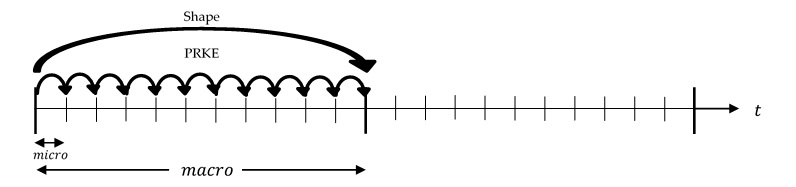
\includegraphics[width=\linewidth]{\FiguresDir/IQS_visualization.jpg}
\caption{IQS method visualization}
\label{fig:iqsviz}
\end{figure}

By this design, the benefits of IQS is most realized when using time adaptive techniques, one of these is described in Section \ref{sect:dt2}.  As we noted earlier, shape-PRKE equations are a nonlinear system and thus need to be solved in a iterative manner.  Each macro time step can be iterated so the best shape is used to compute power at the micro time steps.  This iteration process must converge the shape such that the uniqueness condition $(\frac{d}{dt}\sum_{g=1}^G\left(\phi^{*g},\frac{1}{v^g}\varphi^g\right)=0)$ is preserved.  The most convenient method to implement in Rattlesnake are Picard iterations.  Where initially, the shape is evaluated with a guessed amplitude, if the normalization condition changes significantly, then the PRKE is evaluated with parameters computed from the last solution.  This process is repeated until convergence.  Picard iteration is predominantly utilized for multiphysics simulation, where neutronics is nonlinearly coupled to thermal-hydraulics.  So the shape-PRKE couple is easily fit into this process, described by Figure \ref{fig:picard}.

\begin{figure}[!htpb]
\centering
\begin{tikzpicture}[every node/.style = {font=\normalsize}]

\node[greenblock](p1) at (0,0) {Solve shape equations \\ over macro time step};
\node[greenblock](p2) at (0,-2.5) {Compute PRKE parameters \\ over macro time step};
\node[greenblock](p3) at (0,-5) {Solve PRKE using micro \\ steps};
\node[greenblock](p4) at (0,-7.5) {Update $p$ and $\frac{dp}{dt}$};
\node[blueblock] (p5) at (0,-11) {Solve other physics \\ components};
\node[reddiamond] (check) at (0,-15) {Check for \\ convergence};
\node [above =0.1mm of p1] {\large{IQS Solve:}};
\node [above =0.1mm of p5] {\large{Multi-physics:}};

\tikzback{p1}{p1}{p4}{p4}{bk1}
\tikzback{p5}{p5}{p5}{p5}{bk2}

\draw[->,ultra thick](p1.south) -- (p2.north);
\draw[->,ultra thick](p2.south) -- (p3.north);
\draw[->,ultra thick](p3.south) -- (p4.north);
\draw [->,ultra thick] (p4.south)+(0,-0.25) -- node [above] {} (bk2-n);
\draw[->,ultra thick](p5.south)+(0,-0.25) -- (check.north);
%\draw[->,ultra thick](check.west) -- (-5,-15) -- node[above,sloped] {\large{no}}(-5,0) -- node[above] {}(bk1-w);
\draw[->,ultra thick](check.west) -- node[above,sloped] {\large{no}} (-5,-15) |-  node[above] {}(bk1-w);
\draw[->,ultra thick](check.south) -- node[right] {\large{yes}} ++(0,-2);

\end{tikzpicture}
\caption{Visualization of Picard iteration process}
\label{fig:picard}
\end{figure}

%%%%%%%%%%%%%%%%%%%%%%%%%%%%%%%%%%%%%%%%%%%%%%%%
\subsection{A Predictor-Corrector version of IQS (IQS P-C)}
%%%%%%%%%%%%%%%%%%%%%%%%%%%%%%%%%%%%%%%%%%%%%%%%

The Predictor-Corrector version of IQS factorizes the flux and derives the PRKE the same way as the standard version, but the evaluation of the coupled system is different.  This version first solves the flux diffusion (represented by Equations \ref{eq:flux} and \ref{eq:precursor}) to get a predicted flux.  The predicted flux at this step is then converted to shape by rescaling as follows:
\be
\varphi^g_{n+1} = \underbrace{\phi^g_{n+1}}_{\text{predicted}} \frac{K_0}{K_{n+1}}
\label{eq:rescale}
\ee
Where:
\be
K_{n+1} =\sum_{g=1}^G\left(\phi^{*g},\frac{1}{v^g}\phi^g_{n+1}\right)
\ee
\be
K_{0} =\sum_{g=1}^G\left(\phi^{*g},\frac{1}{v^g}\varphi^g_{n+1}\right)=\sum_{g=1}^G\left(\phi^{*g},\frac{1}{v^g}\phi^g_{0}\right)
\ee

The PRKE parameters are then computed with this shape using Equations \ref{eq:rmb} - \ref{eq:l} and interpolated over the macro step, then the PRKE is evaluated.  With the newly computed amplitude, the shape is rescaled and the corrected flux is evaluated:
\be
\underbrace{\phi^g_{n+1}}_{\text{corrected}} = p_{n+1} \times \varphi^g_{n+1}
\ee

The advantage to the predictor-corrector method is there is no iteration necessary for this method and in turn is much simpler and faster than the standard IQS.  The disadvantage is that the method assumes $\sum_{g=1}^G\left(\phi^{*g},\frac{1}{v^g}\varphi^g_{n+1}\right)$ is inherently constant.

%%%%%%%%%%%%%%%%%%%%%%%%%%%%%%%%%%%%%%%%%%%%%%%%
\subsection{Precursor Integration}
\label{sect:prec}
%%%%%%%%%%%%%%%%%%%%%%%%%%%%%%%%%%%%%%%%%%%%%%%%

This section presents two different time-integration methods to solve coupled IQS shape + precursor equations, recalled below using, for simplicity, a single neutron group and a single precursor group.

\be
\frac{1}{v}\frac{\partial\varphi}{\partial t}=\nu\Sigma_f(1-\beta)\varphi-\left(-\div D \grad + \Sigma_a + \frac{1}{v}\frac{1}{p}\frac{dp}{dt}\right)\varphi+\frac{1}{p}\lambda C 
\ee
\be
\frac{dC}{dt} = \beta\nu \Sigma_f \varphi p - \lambda C
\ee

First, we note that we could keep this system of two time-dependent equations and solve it as a coupled system. However, this is unnecessary and a memory expensive endeavor because the precursor equation is only an ODE and not a PDE. Instead, one may discretize in time the shape equation, which typically requires the knowledge of the precursor concentrations at the end of the time step. This precursor value is taken from the solution, numerical or analytical, of the precursors ODE.  \\

Through prototyping, it has been found that typical implicit nor Crank-Nicholson time discretizations of precursors are not preferable methods for solving the shape equation in IQS.  It has been found that these discretizations result in a lack of convergence of the shape over the IQS iteration process.  In order to remedy the error, a analytical representation of the precursors was implemented in the prototype and the shape solution was able to converge.  The method entails linearly interpolating the fission source ($S_f = \nu \Sigma_f \varphi$) and integrating the resulting continuous function analytically. Equation \ref{eq:c_dis} is the equation to solve for the precursors and Equations \ref{eq:a1} and \ref{eq:a2} are integrating factors.

\be
C^{n+1} = C^n e^{-\lambda \Delta t} 
+ \beta_i \left(a_2 S_f^{n+1} + a_1 S_f^{n}\right)
\label{eq:c_dis}
\ee

\be
a_1 = \int_{t_n}^{t_{n+1}}\left(\frac{t_{n+1}-t'}{\Delta t}\right)p(t')e^{-\lambda(t_{n+1}-t')}dt'
\label{eq:a1}
\ee
\be
a_2 = \int_{t_n}^{t_{n+1}}\left(\frac{t'-t_n}{\Delta t}\right)p(t')e^{-\lambda(t_{n+1}-t')}dt'
\label{eq:a2}
\ee

The amplitude $(p)$ is included in the integration coefficient because it has been highly accurately calculated in the micro step scheme, so a piecewise interpolation between those points can be done to maximize accuracy.  


%%%%%%%%%%%%%%%%%%%%%%%%%%%%%%%%%%%%%%%%%%%%%%%%
\subsection{Time Adaptation}
\label{sect:dt2}
%%%%%%%%%%%%%%%%%%%%%%%%%%%%%%%%%%%%%%%%%%%%%%%%

A very important aspect of IQS is how it performs with time adaptation because this will most likely be used with IQS.  The time adaptation used for quantifying IQS's ability is step doubling.  The step doubling technique involves estimating the local error for a certain time step by taking the difference between a solution with one full step and a solution with two half steps.  If the step is small enough, the error will be smaller than a user driven tolerance and the magnitude of the next step will be calculated based on the error.  If the step is too large, the step will be repeated with a smaller step calculated with the resulting error.  The error of the time step is approximated by Equation \ref{eq:edt2}, where $\varphi^g_1$ and $\varphi^g_2$ are the solutions with the full step and half step, respectively.  $\varphi$ is changed to $\phi$ for regular flux evaluation and IQS P-C.  If $e_n > e_{max}$ the time step is repeated; if $e_n < e_{max}$ the system moves to the next time step.  The next $\Delta t$ is calculated using Equation \ref{eq:dt2}, where $\mu$ is the convergence order of the time integration scheme being used.  $e_{max}$ and $e_{tol}$ are user defined parameters; $e_{max}$ is usually less than $e_{tol}$ to better guarantee that the calculated $\Delta t_{new}$ will pass the error criteria so time steps won't be repeated.

\be
e_n = \frac{\norm{\sum_{g=1}^G\varphi^g_2 - \sum_{g=1}^G\varphi^g_1}}{\text{max}\left(\norm{\sum_{g=1}^G\varphi^g_2},\norm{\sum_{g=1}^G\varphi^g_1}\right)}
\label{eq:edt2}
\ee
\be
\Delta t_{new} = \Delta t_{old} \left(\frac{e_{tol}}{e_n}\right)^{\frac{1}{1+\mu}}
\label{eq:dt2}
\ee

To be clear, each solution undergoes Picard iterations until $Error_{IQS}$ converges before the error is calculated; for IQS P-C, each solution is re-scaled by $p$.  Additionally, if the PJFNK iteration does not converge, the entire step doubling process is repeated with half the time original time step. 

%%%%%%%%%%%%%%%%%%%%%%%%%%%%%%%%%%%%%%%%%%%%%%%%
%%%%%%%%%%%%%%%%%%%%%%%%%%%%%%%%%%%%%%%%%%%%%%%%
\section{Rattlesnake Implementation}
%%%%%%%%%%%%%%%%%%%%%%%%%%%%%%%%%%%%%%%%%%%%%%%%
%%%%%%%%%%%%%%%%%%%%%%%%%%%%%%%%%%%%%%%%%%%%%%%%

Rattlesnake is a MOOSE-based application developed INL specific to solving radiation transport problems with multiphysics capabilities.  MOOSE is a finite-element based, multiphysics framework that gives the general architecture for the development of physics application like Rattlesnake.  Because radiation transport is such a complex problem, Rattlesnake is a relatively large application with a lot of functionality.  At the heart of Rattlesnake is the action system.  The Rattlesnake action system gives the capability of consolidating MOOSE input syntax, so that a user does not have to define every kernel, variable, etc. in the problem, which could be on the order of thousands with multi-group problems.  The user, instead, is able to input an equation description (Diffusion, S$_n$, P$_n$, etc.) and solve method (SAAF,LS,CFEM,DFEM,etc.), and the action system will incorporate all the necessary physics involved (kernels, boundary conditions, postprocessor, etc.).

 
%%%%%%%%%%%%%%%%%%%%%%%%%%%%%%%%%%%%%%%%%%%%%%%%
\subsection{Executioner}
%%%%%%%%%%%%%%%%%%%%%%%%%%%%%%%%%%%%%%%%%%%%%%%%

The IQS executioner derives from the Transient executioner in MOOSE.  The IQS executioner contains a loop over micro time steps that computes the PRKE and then passes $p$ and $\frac{dp}{dt}$ for the Transient executioner to evaluate the shape equation at each macro step.  The PRKE is computed with a user specified option of backward-Euler, Crank-Nicolson, or SDIRK33.   The IQS executioner also supplements Transient Picard iteration process by adding its own error criteria:
\be
Error_{IQS}=\left|\frac{\sum_{g=1}^G\left(\phi^{*g},\frac{1}{v^g}\varphi^{g,n}\right)}{\sum_{g=1}^G\left(\phi^{*g},\frac{1}{v^g}\varphi^{g,0}\right)}-1\right|
\label{eq:eiqs}
\ee

%%%%%%%%%%%%%%%%%%%%%%%%%%%%%%%%%%%%%%%%%%%%%%%%
\subsection{Action System}
%%%%%%%%%%%%%%%%%%%%%%%%%%%%%%%%%%%%%%%%%%%%%%%%

IQS defines its uniqueness from its executioner type; however, many changes needed to be made in the Rattlesnake action system in order to support IQS execution.   First, changes needed to be made in order to evaluate the shape equation.  The shape equation, after some manipulation, is very similar to the time-dependent, which Rattlesnake is already set up to solve:

\begin{align}
\frac{1}{v^g}\frac{\partial\varphi^g}{\partial t}=&\underbrace{\frac{\chi_p^g}{\keff} \sum_{g'=1}^G (1-\beta) \nu^{g'} \Sigma_f^{g'} \varphi^{g'}}_{Flux Kernel} + \underbrace{\sum_{g'\neq g}^G\Sigma_s^{g'\to g} \varphi^{g'}}_{Flux Kernel} - \underbrace{\left( -\div D^g \grad \right)\varphi^g}_{Flux Kernel} - \underbrace{\Sigma_r^g\varphi^g}_{Flux Kernel} \nonumber \\
& - \underbrace{\frac{1}{v^g} \overbrace{\frac{1}{p}\frac{dp}{dt}}^{From Executioner}\varphi^g}_{IQS Kernel}+\underbrace{\frac{1}{p}\sum_{i=1}^I\chi_{d,i}^g\lambda_iC_i}_{Modified Flux Kernel}
\end{align}

To enable Rattlesnake to solve this equation, another kernel was created that evaluates $\sum_{g=1}^G\frac{1}{v^gp}\frac{dp}{dt}\varphi^g$ and added when the IQS executioner is called.  Also, the precursor kernel was modified to include the $\frac{1}{p}$ term. Finally, the precursor auxkernel that evaluates Equation \ref{eq:preq2} using the analytical integration method described in Section \ref{sect:prec}.

%%%%%%%%%%%%%%%%%%%%%%%%%%%%%%%%%%%%%%%%%%%%%%%%
\subsection{PRKE coefficients}
%%%%%%%%%%%%%%%%%%%%%%%%%%%%%%%%%%%%%%%%%%%%%%%%

In order to evaluate the PRKE coefficients, defined by Equations \ref{eq:rmb} - \ref{eq:l}, four postprocessors were created.  The parameter calculations were separated by $\frac{\bar{\beta}_i}{\Lambda}$ numerator, $\bar{\lambda}_i$ numerator/denominator, $\frac{\rho-\bar{\beta}}{\Lambda}/\frac{\bar{\beta}}{\Lambda}$ denominator, and $\frac{\rho-\bar{\beta}}{\Lambda}$ numerator. The first three are relatively simple, only relying on material properties and solution quantities, then computing the elemental integral.  The $\frac{\rho-\bar{\beta}}{\Lambda}$ numerator requires the use of the MOOSE \texttt{save\_in} feature. This feature saves the residual from a calculated kernel or boundary contribution in the shape evaluation to an auxiliary variable.  The postprocessor then computes the inner product of this variable and the initial adjoint solution.  After each of these postprocessors are evaluated, a user object pulls together all the values and performs the numerator/denominator divisions.  The resulting values are then passed to the executioner for the PRKE evaluation.

%%%%%%%%%%%%%%%%%%%%%%%%%%%%%%%%%%%%%%%%%%%%%%%%
\subsection{Other Action Systems}
%%%%%%%%%%%%%%%%%%%%%%%%%%%%%%%%%%%%%%%%%%%%%%%%

For simplicity, IQS implementation has only been described for CFEM diffusion.  However, Rattlesnake has other action systems capable of transient simulation, where IQS can be implemented and be effective.  One of these action systems is DFEM diffusion, where the only major difference from CFEM is the diffusion term in Equation \ref{eq:flux} and \ref{eq:shape2}.  However, in the derivation for IQS is term is unaffected between shape and flux evaluation.  So saving the residual for this diffusion kernel in the \texttt{save\_in} variable is the only alteration to this action for IQS to function.

Additional action systems involve transport, but it is evident from Section \ref{sect:transport} that IQS implementation in these is straightforward.  The main differences between diffusion implementation in transport is outlined below:
\begin{enumerate}
\item The form of the operators in the shape equations is different, but Rattlesnake has already implemented all the kernels necessary to represent these operators.  So no change is necessary to these kernels is necessary for IQS.  Additionally, the $\frac{1}{v^g}\frac{1}{p}\frac{dp}{dt}$ is the same, so both actions can use the same kernel.
\item The PRKE parameters also change because of the operators.  For the $(\rho-\bar{\beta})$ parameter, the same post-processor can be used with the \texttt{save\_in} functionality in MOOSE.  The post-processor for $\bar{\beta}_i$ must be re-written for transport, but takes a very similar form as diffusion.
\end{enumerate}

IQS plans to be available to any action system capable of transient simulation, which include:
\begin{itemize}
\item CFEM-Diffusion
\item DFEM-Diffusion
\item SAAF-CFEM-SN
\item SAAF-CFEM-PN
\item LS-CFEM-SN
\item DFEM-SN
\end{itemize}

%%%%%%%%%%%%%%%%%%%%%%%%%%%%%%%%%%%%%%%%%%%%%%%%
\subsection{Predictor-Corrector Modification}
%%%%%%%%%%%%%%%%%%%%%%%%%%%%%%%%%%%%%%%%%%%%%%%%

In order to preserve the already implemented standard version of IQS, an option in the IQS executioner was created to specify which method is desired.  Because the diffusion solve is flux instead of shape, when predictor-corrector option is specied, the IQS removal kernel ($\frac{1}{v^g}\frac{1}{p}\frac{dp}{dt}$) and the modified precursor kernel are bypassed, while all the postprocessors are still executed.  However, it is difficult to rescale the flux to shape before the PRKE parameter postprocessor are executed.  So the parameters are computed using the full flux, but amplitude is space independent and comes out of the integrals.  As seen in parameter definitions, when shape is replaced with flux, the amplitude comes out of the integral and cancels out.  So the conversion of the predicted flux in Equation \ref{eq:rescale} to shape is unnecessary if the corrected flux is solved with Equation \ref{eq:phicorr2}.  After obtaining the corrected flux, the precursors are re-evaluated using a \texttt{EXEC\_LINEAR}.
\be
\underbrace{\phi^g_{n+1}}_{\text{corrected}} = \underbrace{\phi^g_{n+1}}_{\text{predicted}} \frac{K_0}{K_{n+1}} p_{n+1}
\label{eq:phicorr2}
\ee

%%%%%%%%%%%%%%%%%%%%%%%%%%%%%%%%%%%%%%%%%%%%%%%%
\subsection{Input}
%%%%%%%%%%%%%%%%%%%%%%%%%%%%%%%%%%%%%%%%%%%%%%%%

The input deck for IQS is very similar to the current transient diffusion input file.  The IQS input has a different executioner type and parameters.  The executioner type is simply IQS and input parameters include number of micro time steps, IQS error tolerance, and initial power.  The Rattlesnake transient action system currently requires a multi-app and transfer to compute and pass the initial $\phi$ and $\keff$, which is present in the transient input deck.  However, IQS also requires an initial evaluation of the adjoint flux, for the weighting function.  So another input file and multi-app transfer was made for the adjoint calculation.  \\

Below is the syntax for the executioner block for an IQS input file.  The \texttt{predictor\_corrector} logical determines whether to do IQS P-C or regular IQS.  The \texttt{IQS\_error\_tol} is the tolerance for the IQS error represented by Equation \ref{eq:eiqs} and will at most \texttt{picard\_max\_its} iterations until convergence.  The \texttt{prke\_scheme} defines the time discretization used for the PRKE evaluation. Where \texttt{RK} is SDIRK33, \texttt{CN} is Crank-Nicholson, and \texttt{IE} is implicit-Euler.
\begin{lstlisting}
[Executioner]
  type = IQS
  predictor_corrector = true/false
  picard_max_its = 5
  ...
  n_micro = 10000
  IQS_error_tol = 1e-7
  prke_scheme = 'RK'
[]
\end{lstlisting}

Since IQS needs to use the adjoint solution for the PRKE parameter evaluation, auxiliary variables need to be created for each group in the input file.  Below is an example of their definition:
\begin{lstlisting}
[AuxVariables]
  [./adjoint_flux_g0]
    family = LAGRANGE
    order = FIRST
  [../]
  [./adjoint_flux_g1]
    family = LAGRANGE
    order = FIRST
  [../]
  ...
[]
\end{lstlisting}

Below is the syntax for the multi-app block to perform forward and adjoint steady-state evaluations:
\begin{lstlisting}
[MultiApps]
 [./initial_solve]
   type = FullSolveMultiApp
   execute_on = initial
   input_files = initial.i
 [../]
 [./adjoint_solve]
   type = FullSolveMultiApp
   execute_on = initial
   input_files = adjoint.i
 [../]
[]
\end{lstlisting}

Below is the syntax for the Transfer block to copy the initial and adjoint solutions from the multi-apps.
\begin{lstlisting}
[Transfers]
 [./copy_solution]
   type = TransportSystemVariableTransfer
   direction = from_multiapp
   multi_app = initial_solve
   execute_on = initial
   from_transport_system = diff
   to_transport_system = diff
 [../]
 [./copy_adjoint]
   type = MultiAppVariableTransfer
   execute_on = initial
   direction = from_multiapp
   multi_app = adjoint_solve
   from_variables = 'sflux_g0 sflux_g1 ...'
   to_variables = 'adjoint_flux_g0 adjoint_flux_g1 ...'
 [../]
 [./copy_eigenvalue]
   type = EigenvalueTransfer
   execute_on = initial
   direction = from_multiapp
   multi_app = initial_solve
 [../]
[]
\end{lstlisting}


\newpage
%------------------------------------------------------------------------------
%
%------------------------------------------------------------------------------
%%%%%%%%%%%%%%%%%%%%%%%%%%%%%%%%%%%%%%%%%%%%%%%%
%%%%%%%%%%%%%%%%%%%%%%%%%%%%%%%%%%%%%%%%%%%%%%%%
\section{RESULTS} 
\label{sect::results}
%%%%%%%%%%%%%%%%%%%%%%%%%%%%%%%%%%%%%%%%%%%%%%%%
%%%%%%%%%%%%%%%%%%%%%%%%%%%%%%%%%%%%%%%%%%%%%%%%

This section describes results of an examples that tests the IQS implementation and shows its effectiveness on computation speed and accuracy.  Three examples were selected for this purpose.  The first is a homogeneous one-group problem, subjected to a heterogeneous material change (absorption cross-section change as a ramp in time for a subset of the geometry).  The second is the two-dimensional TWIGL ramp transient benchmark, described further.  The final is the LRA benchmark, which a two-dimensional, temperature feedback example.  Each example was solved with regular diffusion (brute force), IQS, and IQS P-C.  Each method was tested with backward-Euler and BDF2 for the first two examples; just Crank-Nicholson was used for third example.  The performance for each method are represented by convergence plots with constant $\Delta t$ and by the number of time steps with step doubling time adaptation.

%%%%%%%%%%%%%%%%%%%%%%%%%%%%%%%%%%%%%%%%%%%%%%%%
\subsection{One-Dimensional Custom Example}
%%%%%%%%%%%%%%%%%%%%%%%%%%%%%%%%%%%%%%%%%%%%%%%%

The example is very simple and computes quickly, it entails a one dimensional, heterogeneous 400 cm slab with a varying absorption cross section.   Figure \ref{fig:slab} how the regions of the slab are divided and Table \ref{tab:1Dmat} shows the initial material properties.  Regions 2, 3, and 4 have slope perturbations at different points in time, Table \ref{tab:1Dslope} shows the values of the absorption cross-section in each region at the times of interest.  The values of $\Sigma_a$ between these times of interest are linear interpolations between the given values.

\begin{figure}[!htbp]
\begin{center}
\begin{tabular}{| l | l | l | l | l | l | l | l | l | l | l | l | l | l | l | l | l | l | l | l |}
\hline \hline \hline
  &   &   &   &   &   &    &    &   &   &   &   &   &   &   &   &   &   &   &   \\
1 & 1 & 1 & 1 & 2 & 3 & 1 & 1 & 1 & 1 & 1 & 1 & 1 & 1 & 4 & 4 & 1 & 1 & 1 & 1 \\
  &   &   &   &   &   &    &    &   &   &   &   &   &   &   &   &   &   &   &   \\
\hline \hline \hline
\end{tabular}
\caption{1-D heterogeneous slab region identification}
\label{fig:slab}
\end{center}
\end{figure}

\begin{table}[!htbp]
\begin{center}
\caption{1-D heterogeneous slab material properties and problem parameters}
\label{tab:1Dmat}
\begin{tabular}{llllll}
\hline
$D (cm)$ & $\Sigma_a (cm^{-1})$ & $\nu \Sigma_f (cm^{-1})$ & $v (cm/s)$ & $\beta$ & $\lambda (s^{-1})$ \\
\hline
1.0 & 1.1 & 1.1 & 1,000 & 0.006 & 0.1 \\

\hline
\end{tabular}
\end{center}
\end{table}

\begin{table}[!htbp]
\begin{center}
\caption{1-D heterogeneous slab absorption cross-section at times of interest}
\label{tab:1Dslope}
\begin{tabular}{llllllll}
\hline
Region & Material Property & 0.0 s & 0.1 s & 0.6 s & 1.0 s & 1.7 s \\
\hline
2 & $\Sigma_{a} (cm^{-1})$ & 1.1 & 1.1 & 1.095 & 1.095 & 1.095 \\
3 & $\Sigma_{a} (cm^{-1})$ & 1.1 & 1.1 & 1.09 & 1.09 & 1.1 \\
4 & $\Sigma_{a} (cm^{-1})$ & 1.1 & 1.1 & 1.105 & 1.105 & 1.105 \\
\hline
\end{tabular}
\end{center}
\end{table}



Figure \ref{fig:power} shows the power at each macro time step as compared to the traditional brute force (full flux time discretization) method.  The strong correlation between the two curves shows that IQS is consistent with a proven method for a highly transient example.  Figure \ref{fig:conv} shows that IQS is not only consistent for this example, but also has a better error constant in the convergence study.  Figure \ref{fig:conv} shows the error convergence for brute force and IQS methods.  This plot shows that IQS has consistent convergence slope for first and second order time schemes and that IQS has a better error constant for the convergence.  Table \ref{tab:1Ddt2} shows the results for time adaptation.  These results show that traditional IQS does not perform well with step doubling time adaptation and IQS P-C performs moderately better than brute force.

%Figures \ref{fig:initial} - \ref{fig:final} plots shape changes in the IQS method, showing where the shape solution is necessary and a simple PRKE evaluation is inadequate.

\begin{figure}[!htbp]
\centering
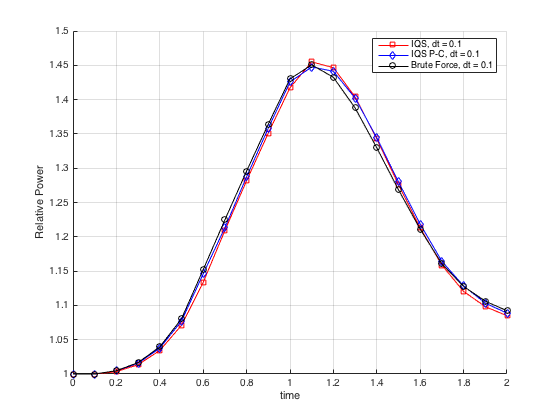
\includegraphics[width=0.49\textwidth]{\FiguresDir/1D_het_power_plot.png}
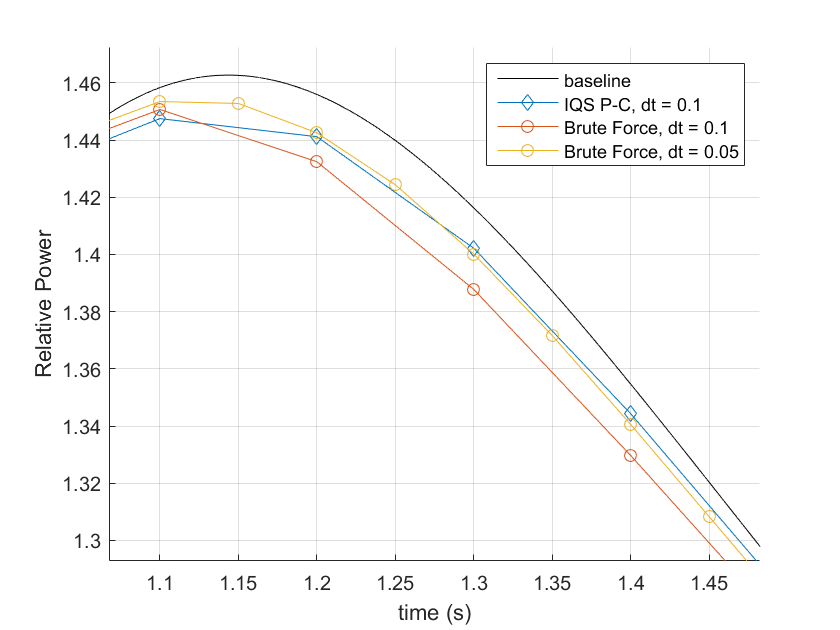
\includegraphics[width=0.5\textwidth]{\FiguresDir/1D_het_power_plot2.png}
\caption{Power level of 1D heterogeneous example}
\label{fig:power}
\end{figure}

%\begin{figure}[!htbp]
%\begin{center}
%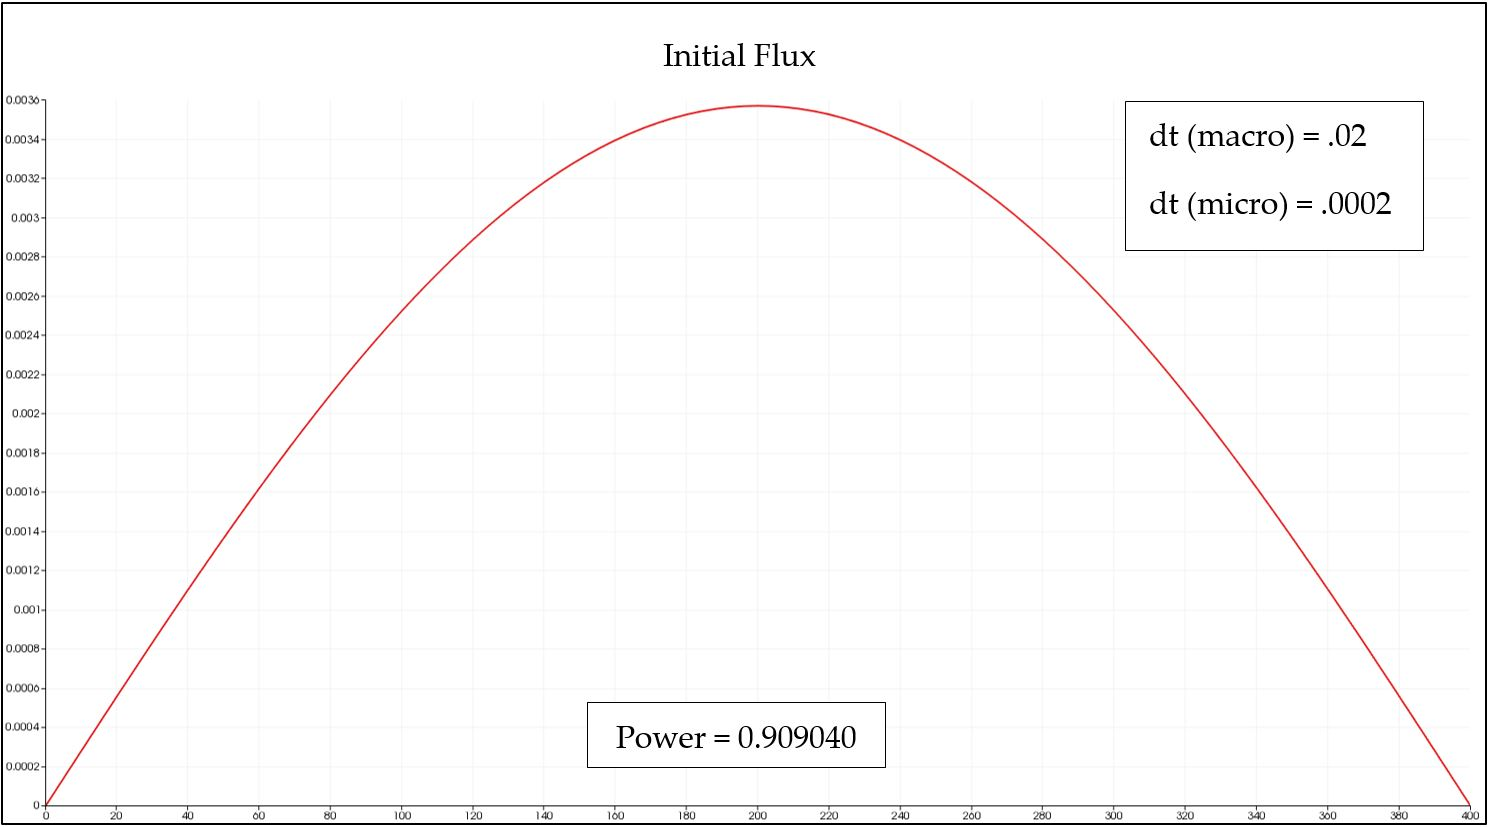
\includegraphics[width=5in,height=2in]{\FiguresDir/initial_flux.jpg}
%\caption{Initial Flux Plot}
%\label{fig:initial}
%\end{center}
%\end{figure}
%
%\begin{figure}[!htbp]
%\begin{center}
%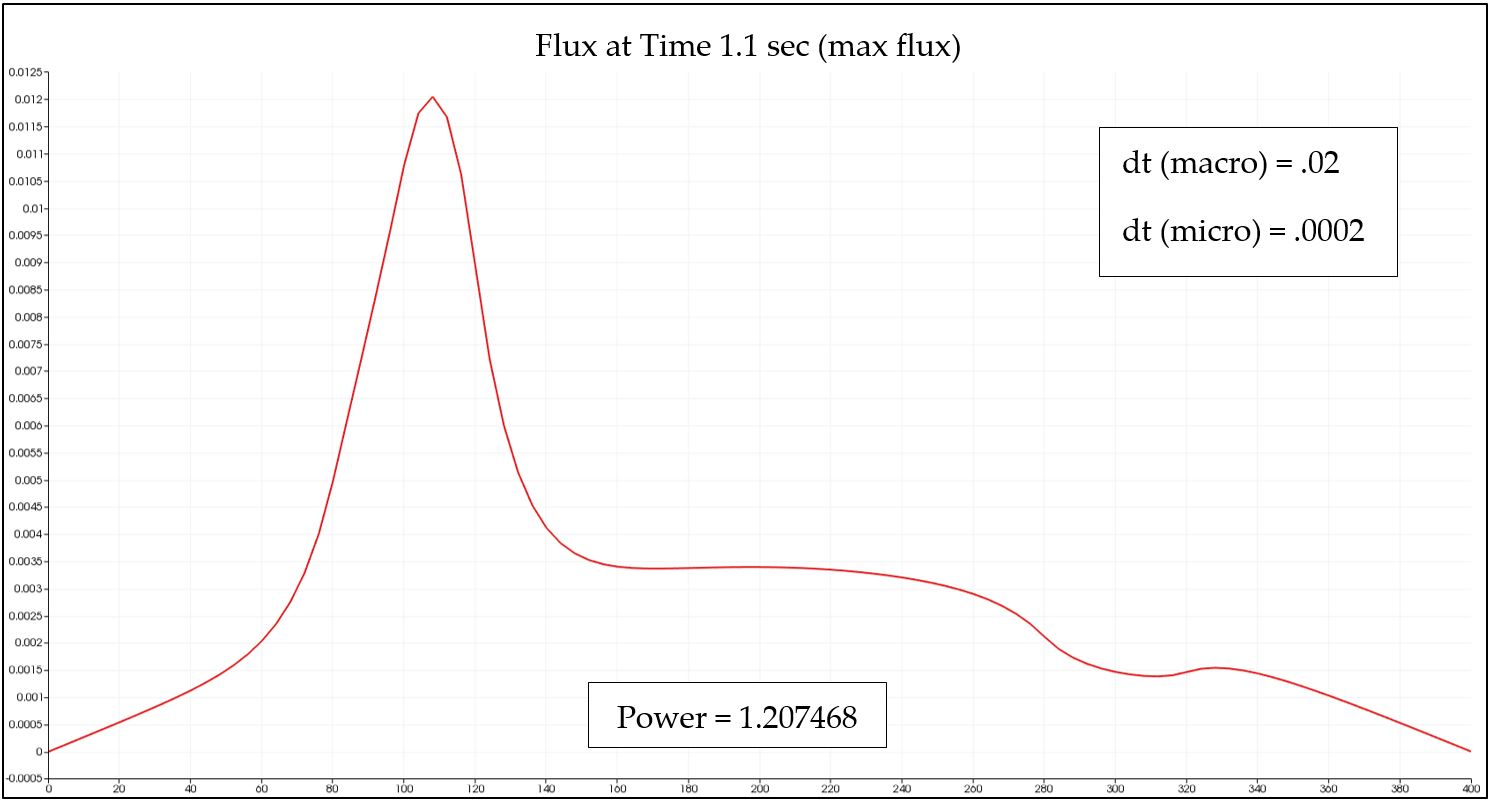
\includegraphics[width=5in,height=2in]{\FiguresDir/max_flux.jpg}
%\caption{Flux Plot when Absorption Cross Section is at Minimum}
%\label{fig:max}
%\end{center}
%\end{figure}
%
%\begin{figure}[!htbp]
%\begin{center}
%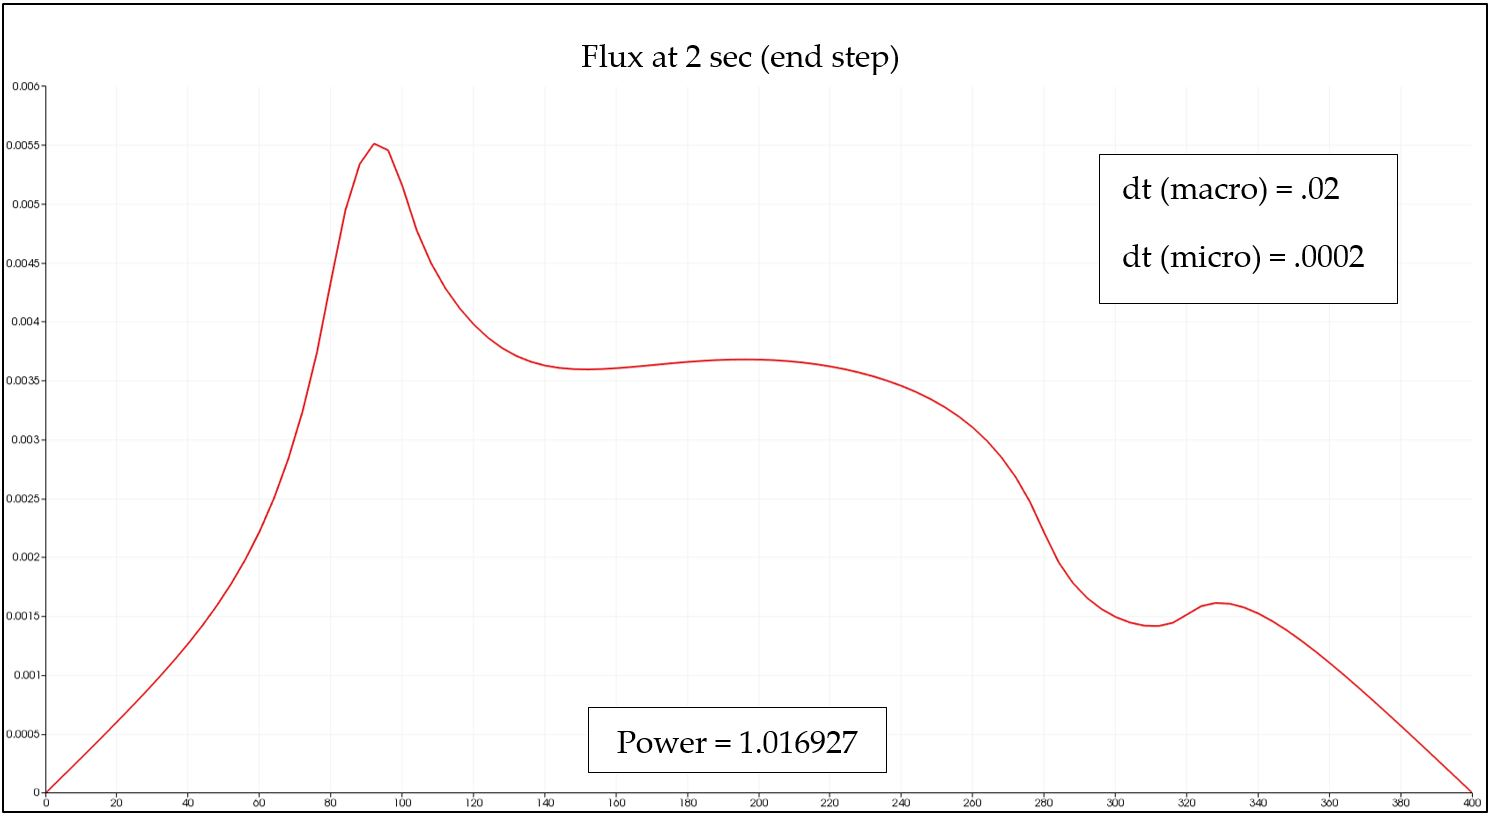
\includegraphics[width=5in,height=2in]{\FiguresDir/final_flux.jpg}
%\caption{Final Flux Computation (not steady-state)}
%\label{fig:final}
%\end{center}
%\end{figure}

\begin{figure}[!htbp]
\centering
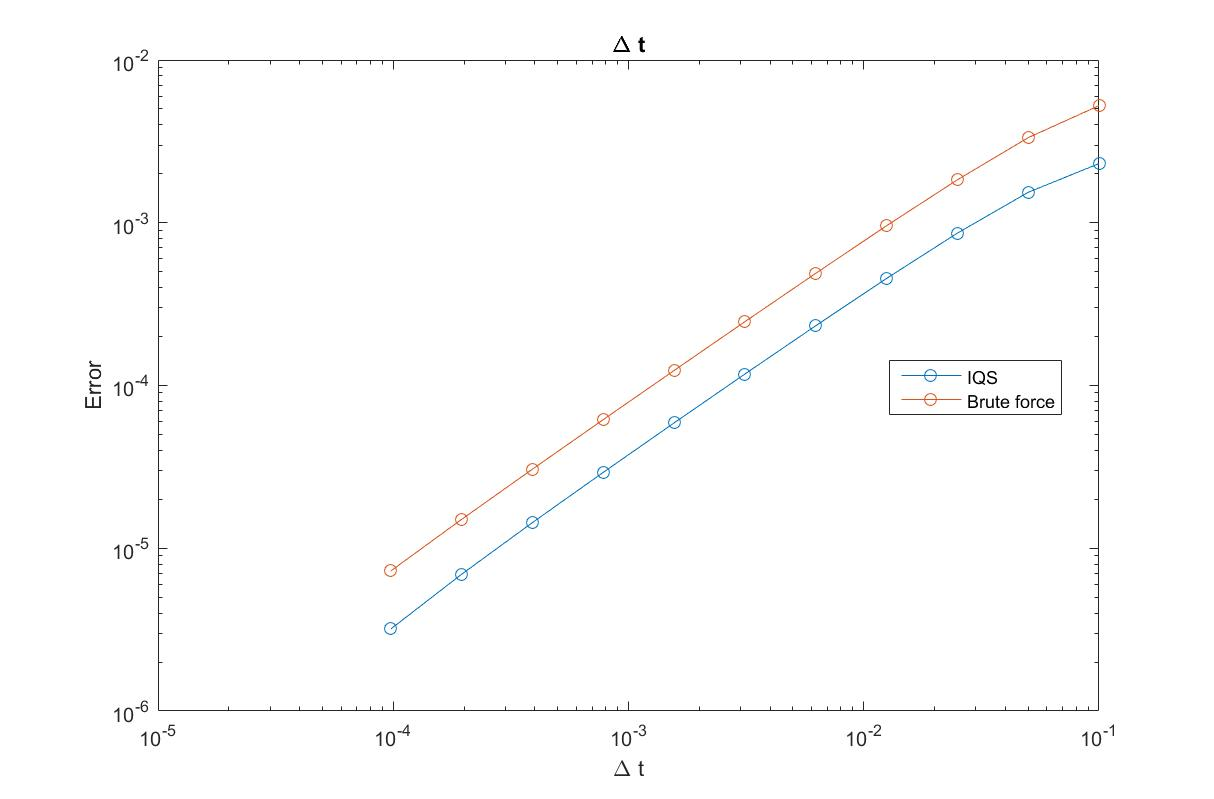
\includegraphics[width=5in]{\FiguresDir/1D_het_convergence.jpg}
\caption{Error convergence comparison of 1D hetergenous example}
\label{fig:conv}
\end{figure}

\begin{table}[!htbp]
\begin{center}
\caption{1-D heterogeneous slab step doubling results}
\label{tab:1Ddt2}
\resizebox{\textwidth}{!}{
\begin{tabular}{|l|l|l|l|l|l|l|l|l|l|l|}
\hline
  &  & \multicolumn{3}{|c|}{Brute Force} & \multicolumn{3}{|c|}{IQS} & \multicolumn{3}{|c|}{IQS P-C} \\
\hline
Test & $e_{max}$ & Error & Steps & Solves & Error & Steps & Solves & Error & Steps & Solves \\
\hline
1 &	0.05 	&	0.021596 &	10  &	32	 &	0.10084 &	12	  &	175		&	0.028019 &	10	&	33 \\
2 &	0.01 	&	0.032864 &	21  &	80	 &	0.08030 &	41	  &	850	 	&	0.044721 &	20	&	74 \\
3 &	0.005 	&	0.053159 &	27  &	96	 &	0.01215 &	115	  &	2220 	&	0.052095 &	25	&	96 \\
4 & 0.001 	&	0.056546 &	56  &	188	 &	0.03242 &	848	  &	12511 	&	0.061274 &	50	&	162 \\
5 &	0.0005 	&	0.062882 &	77  &	245	 &	0.03491 &	1718  &	25841 	&	0.061240 &	69	&	225 \\
6 &	0.0001 	&	0.060089 &	177 &	537	 &	0.03554 &	8702  &	129985 	&	0.060824 &	159	&	480 \\
7 &	5.0e-05	&	0.059513 &	252 &	767	 &	0.03622 &	17282 &	256463 	&	0.061078 &	224	&	680 \\
8 &	1.0e-05	&	0.061063 &	561 &	1691 &	0.03142 &	79988 &	1104227 &	0.061901 &	501	&	1509 \\
\hline
\end{tabular}}
\end{center}
\end{table}

\newpage
%%%%%%%%%%%%%%%%%%%%%%%%%%%%%%%%%%%%%%%%%%%%%%%%
\subsection{TWIGL Benchmark}
%%%%%%%%%%%%%%%%%%%%%%%%%%%%%%%%%%%%%%%%%%%%%%%%

This benchmark problem originates from the Argonne National Lab Benchmark Problem Book \cite{ANL_BPB}.  It is a 2D, 2-group reactor core model with no reflector region shown in Figure \ref{fig:TWIGL_reg}.  Table \ref{tab:TWIGL_mat} shows the material properties of each fuel region and the ramp perturbation of Material 1.

\begin{figure}[!htbp]
\begin{center}
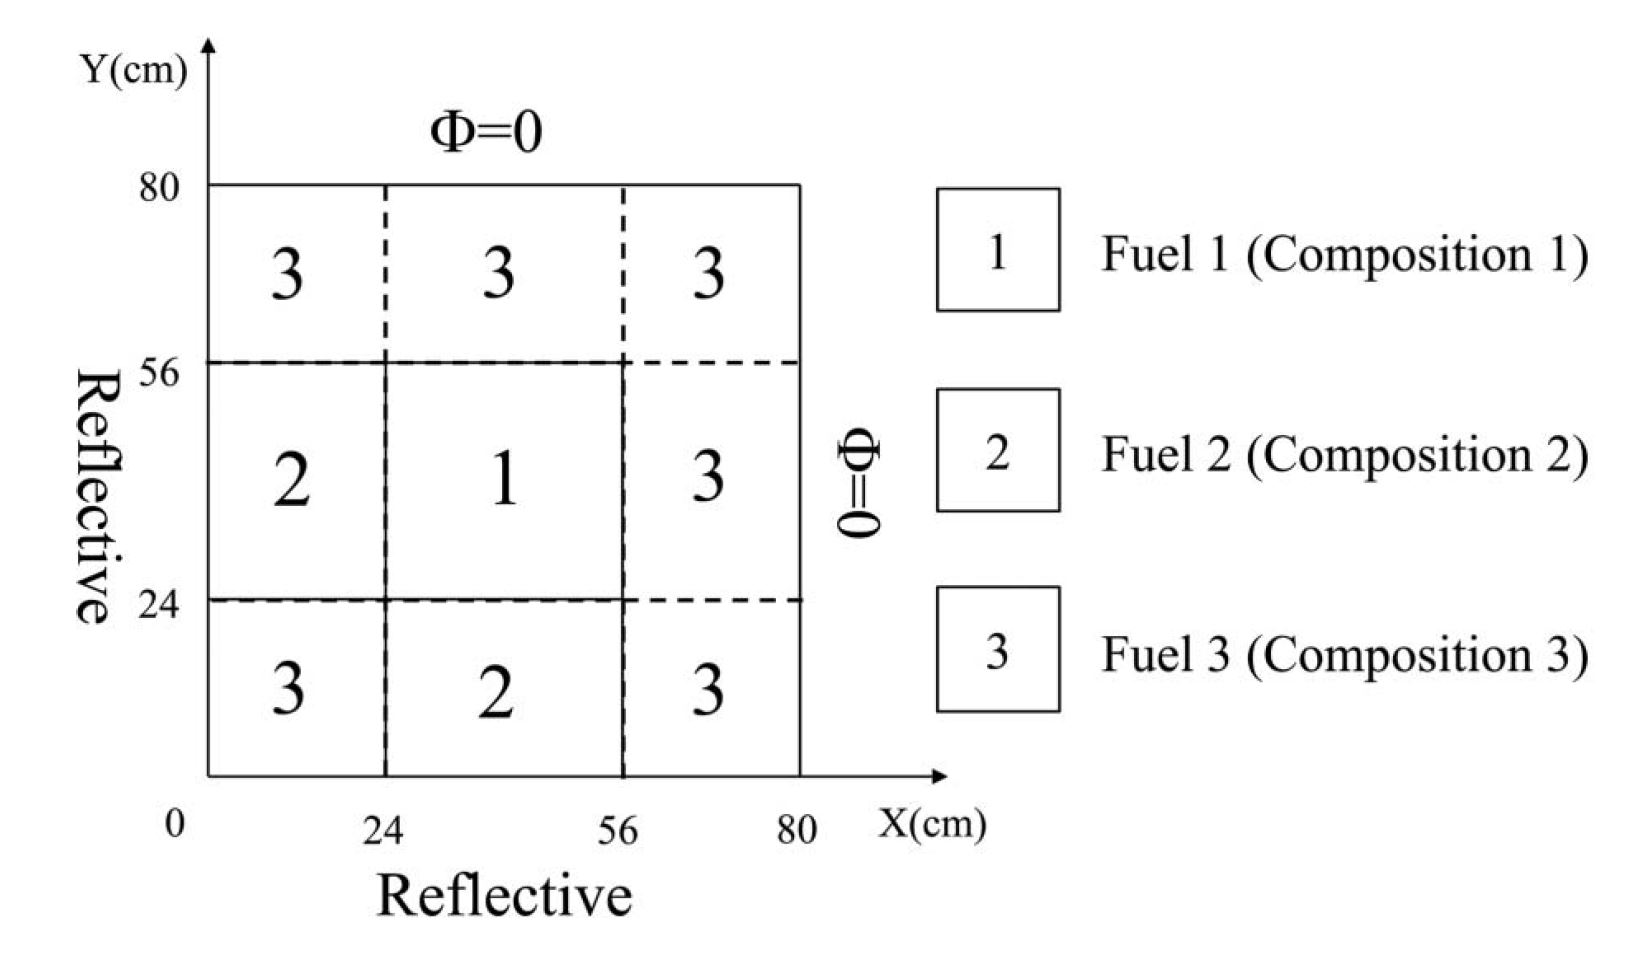
\includegraphics[width=0.75\textwidth]{\FiguresDir/TWIGL_regions.jpg}
\caption{TWIGL benchmark problem description}
\label{fig:TWIGL_reg}
\end{center}
\end{figure}

\begin{table}[!htbp]
\begin{center}
\caption{1-D heterogeneous slab absorption cross-section slope perturbation}
\label{tab:TWIGL_mat}
\begin{tabular}{llllllll}
\hline
  &  &  &  &  &  &  \multicolumn{2}{c}{$\underline{\Sigma_s (cm^{-1})} $} \\
Material & Group & $D (cm)$ & $\Sigma_a (cm^{-1})$ & $\nu\Sigma_f (cm^{-1})$ & $\chi$ & $g \rightarrow 1$ & $g \rightarrow 2$ \\
\hline
1 & 1 & 1.4 & 0.010 & 0.007 & 1.0 & 0.0 & 0.01 \\
  & 2 & 0.4 & 0.150 & 0.200 & 0.0 & 0.0 & 0.00  \\
2 & 1 & 1.4 & 0.010 & 0.007 & 1.0 & 0.0 & 0.01  \\
  & 2 & 0.4 & 0.150 & 0.200 & 0.0 & 0.0 & 0.00  \\
3 & 1 & 1.3 & 0.008 & 0.003 & 1.0 & 0.0 & 0.01  \\
  & 2 & 0.5 & 0.050 & 0.060 & 0.0 & 0.0 & 0.00  \\
\hline
  & $\nu$ & $v_1 (cm/s)$ & $v_2 (cm/s)$ & $\beta$ & $\lambda (1/s)$ &   &   \\
\hline
  & 2.43 & 1.0E7 & 2.0E5 & 0.0075 & 0.08 &   &   \\
\hline
 \multicolumn{8}{l}{\footnotesize Material 1 ramp perturbation:} \\
\multicolumn{8}{l}{\footnotesize $\Sigma_{a,2}(t)=\Sigma_{a,2}(0) \times (1-0.11667t) \quad t \leq 0.2 s$} \\
\multicolumn{8}{l}{\footnotesize $\Sigma_{a,2}(t)=\Sigma_{a,2}(0) \times (0.97666t) \quad t > 0.2 s$} \normalsize
\end{tabular}
\end{center}
\end{table}

Figures \ref{fig:TWIGL_power} show the IQS  solution as compared with the Brute Force solution.  These plots show that IQS is consistent in more complex, higher dimensional problems in Rattlesnake.  Finally, Figure \ref{fig:TWIGL_conv} plots the error convergence of IQS and the Brute Force methods.  The curves show the impressive convergence of IQS for the highly transient TWIGL example.  Table \ref{tab:TWIGLdt2} and Figure \ref{fig:TWIGL_power_dt2} show the results for time adaptation.  The results show that both IQS methods perform exceptionally well compared to brute force.  It also shows that traditional IQS performed better with large $e_{max}$, while IQS P-C was better with smaller $e_{max}$.

%It is important to note the IQS shape plot is scaled differently than the Brute Force flux plot because the amplitude term is not included, but the gradients of colors is comparable.

\begin{figure}[!htbp]
\centering
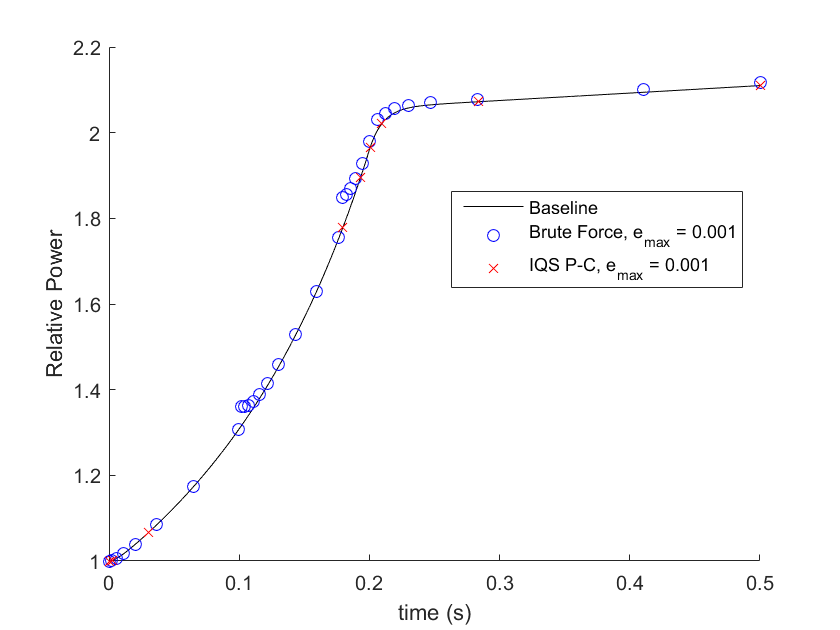
\includegraphics[width=0.49\linewidth]{\FiguresDir/TWIGL_power_plot.png}
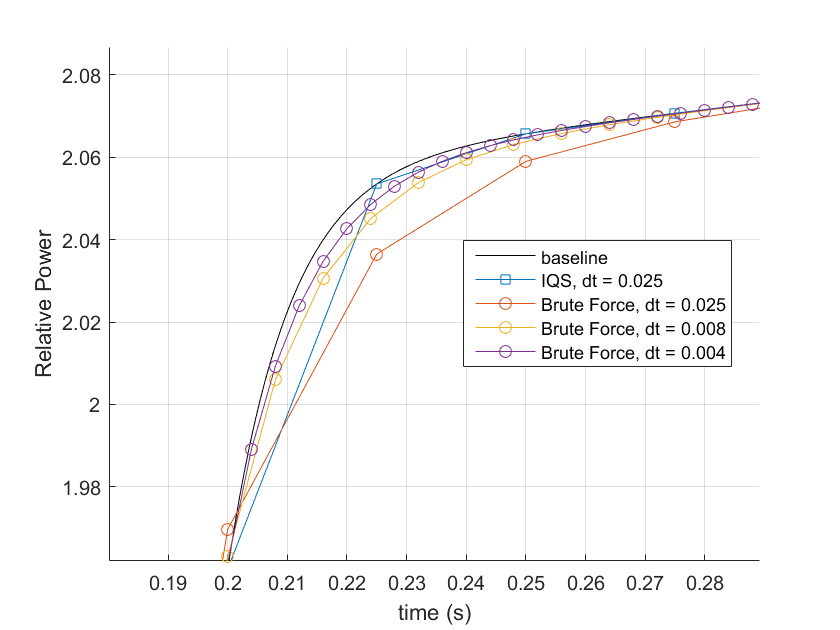
\includegraphics[width=0.5\linewidth]{\FiguresDir/TWIGL_power_plot2.png}
\caption{Power level comparison of TWIGL Benchmark}
\label{fig:TWIGL_power}
\end{figure}

%\begin{figure}[!htbp]
%\begin{center}
%\begin{subfigure}[!htbp]{0.4\textwidth}
%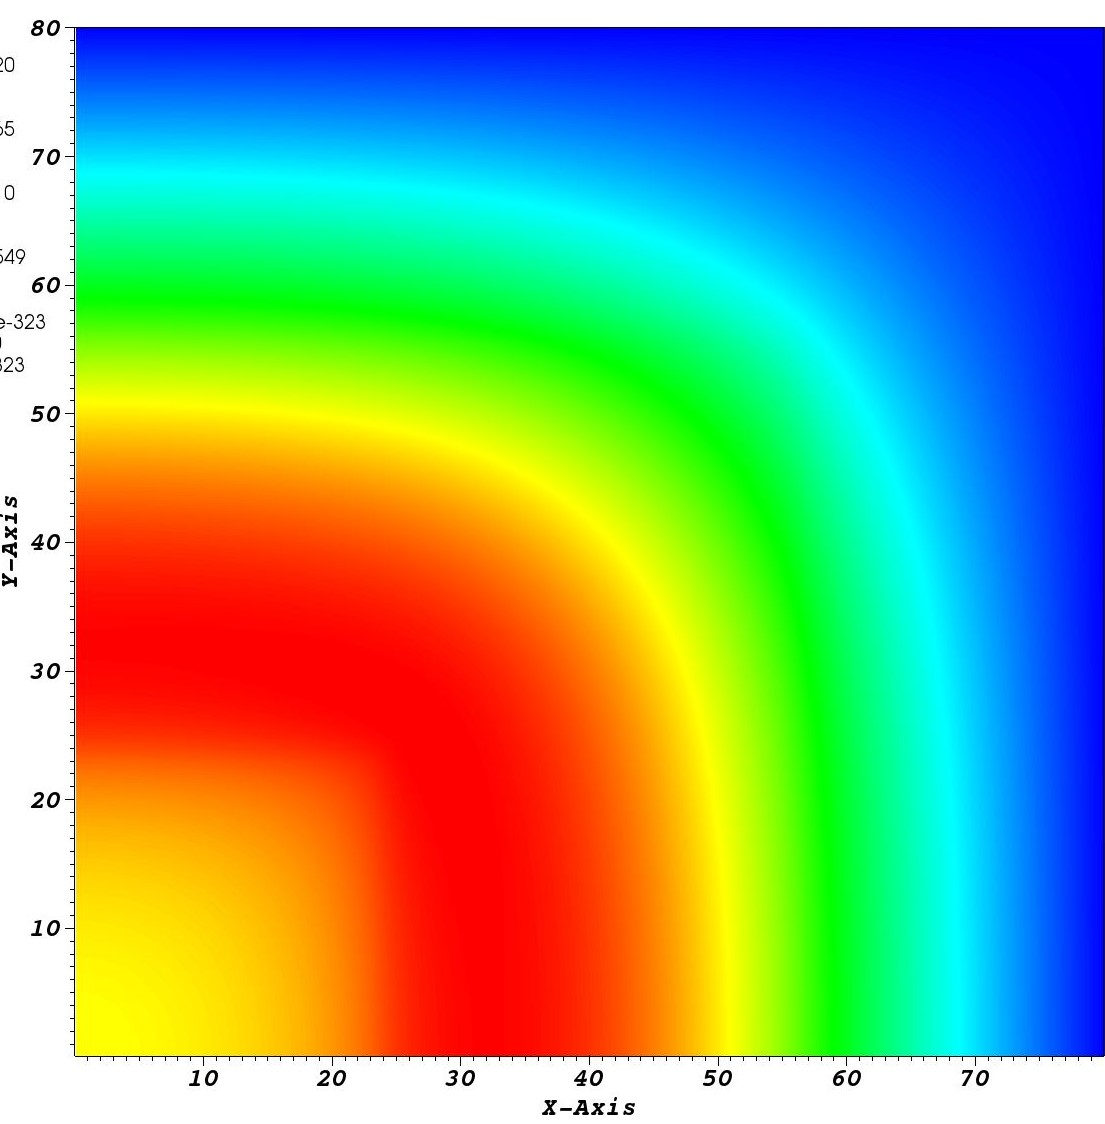
\includegraphics[width=\textwidth]{\FiguresDir/ndiff_ramp_flux.jpg}
%\caption{Brute force flux}
%\end{subfigure}
%\quad
%\begin{subfigure}[!htbp]{0.4\textwidth}
%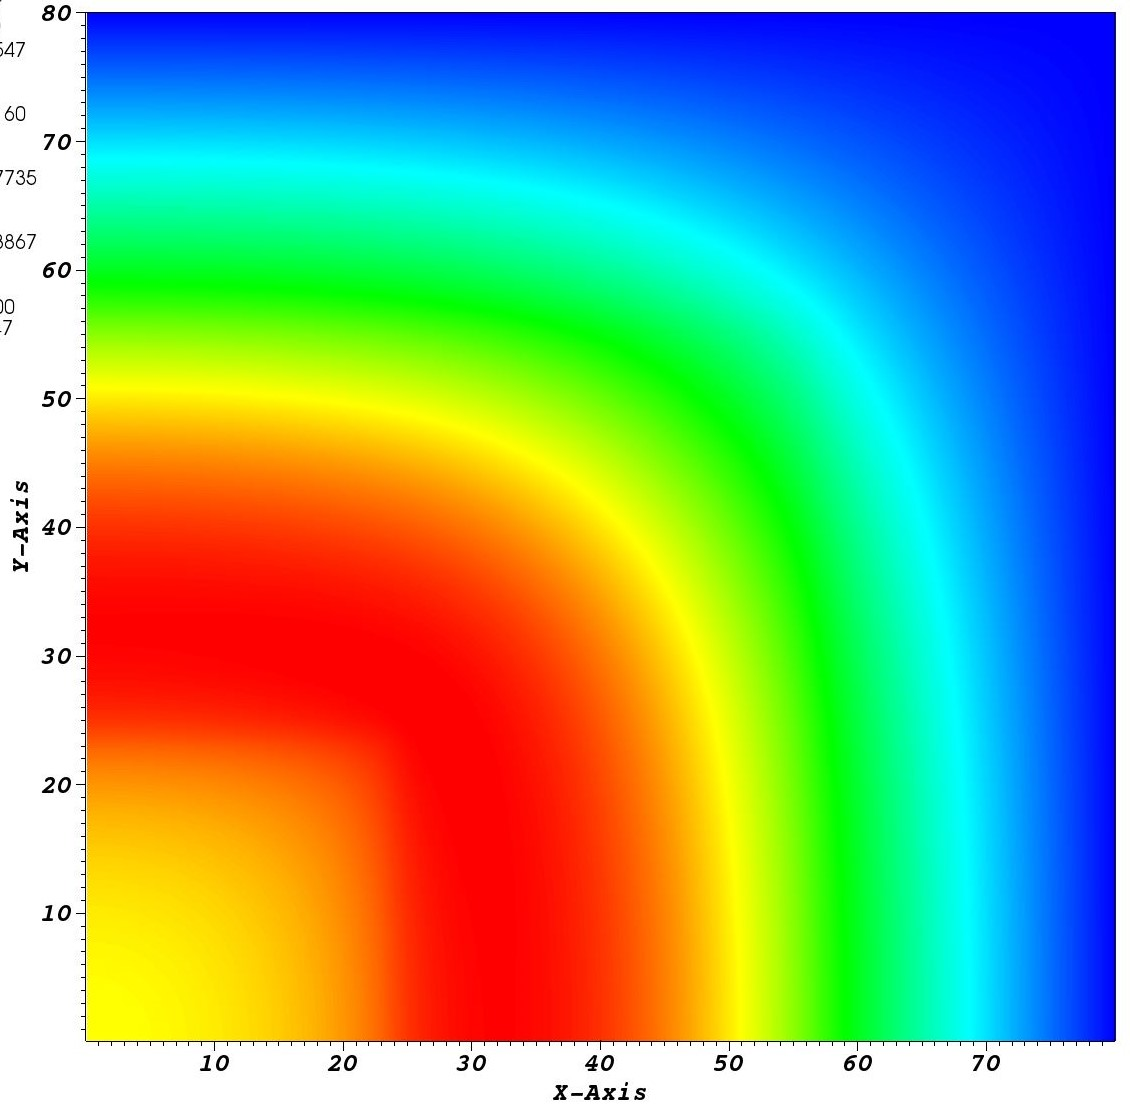
\includegraphics[width=\textwidth]{\FiguresDir/iqs_ramp_shape.jpg}
%\caption{IQS Shape}
%\end{subfigure}
%\caption{TWIGL Benchmark flux/shape comparison at $t=0.2$}
%\label{fig:TWIGL_plots}
%\end{center}
%\end{figure}

\begin{figure}[!htbp]
\centering
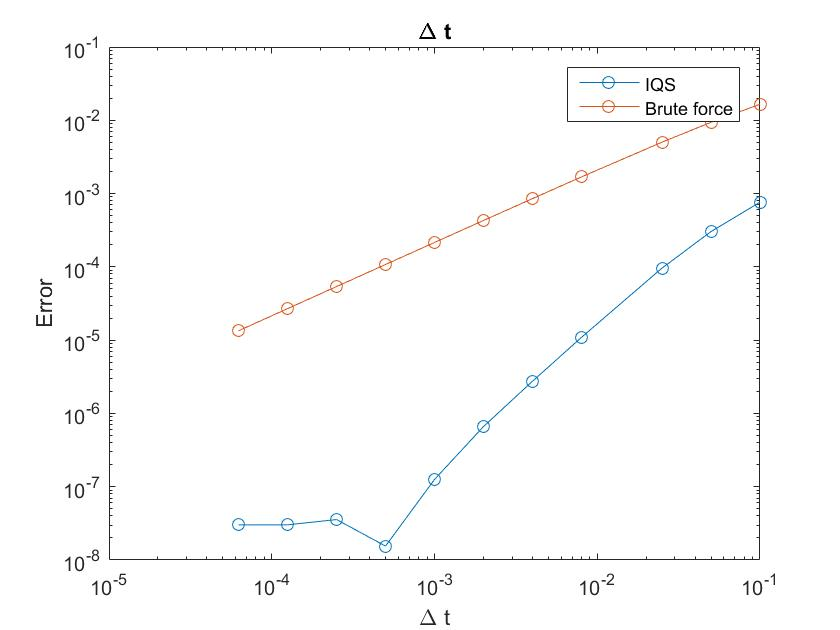
\includegraphics[width=5in]{\FiguresDir/TWIGL_convergence.jpg}
\caption{Error convergence comparison of TWIGL Benchmark}
\label{fig:TWIGL_conv}
\end{figure}

\begin{table}[!htbp]
\begin{center}
\caption{TWIGL step doubling results}
\label{tab:TWIGLdt2}
\resizebox{\textwidth}{!}{
\begin{tabular}{|l|l|l|l|l|l|l|l|l|l|l|}
\hline
  &  & \multicolumn{3}{|c|}{Brute Force} & \multicolumn{3}{|c|}{IQS} & \multicolumn{3}{|c|}{IQS P-C} \\
\hline
Test & $e_{max}$ & Error & Steps & Solves & Error & Steps & Solves & Error & Steps & Solves \\
\hline
1 &	0.05    &	0.00012677 &	9   &	29  &	0.03380433 &	4   &	20   &	0.00323100 &	4  &	9   \\
2 &	0.01    &	3.5555e-05 &	11  &	35  &	0.00166991 &	5   &	40   &	0.00263068 &	5  &	12  \\
3 &	0.005   &	4.0364e-05 &	11  &	31  &	0.00886584 &	5   &	40   &	0.00160486 &	6  &	21  \\
4 &	0.001   &	0.00294822 &	33  &	122 &	0.02976305 &	5   &	36   &	1.7527e-05 &	10 &	35  \\
5 &	0.0005  &	0.00099778 &	39  &	131 &	0.00143781 &	6   &	55   &	1.4185e-05 &	16 &	74  \\
6 &	0.0001  &	0.00019510 &	78  &	236 &	0.00016175 &	7   &	65   &	6.2903e-06 &	19 &	78  \\
7 &	5.0e-05 &	0.00018372 &	112 &	342 &	6.0328e-05 &	12  &	163  &	1.5247e-06 &	24 &	92  \\
8 &	1.0e-05 &	8.0564e-05 &	263 &	794 &	7.7103e-05 &	379 &	5729 &	9.8321e-07 &	48 &	210 \\
\hline

\end{tabular}}
\end{center}
\end{table}

\begin{figure}[!htbp]
\centering
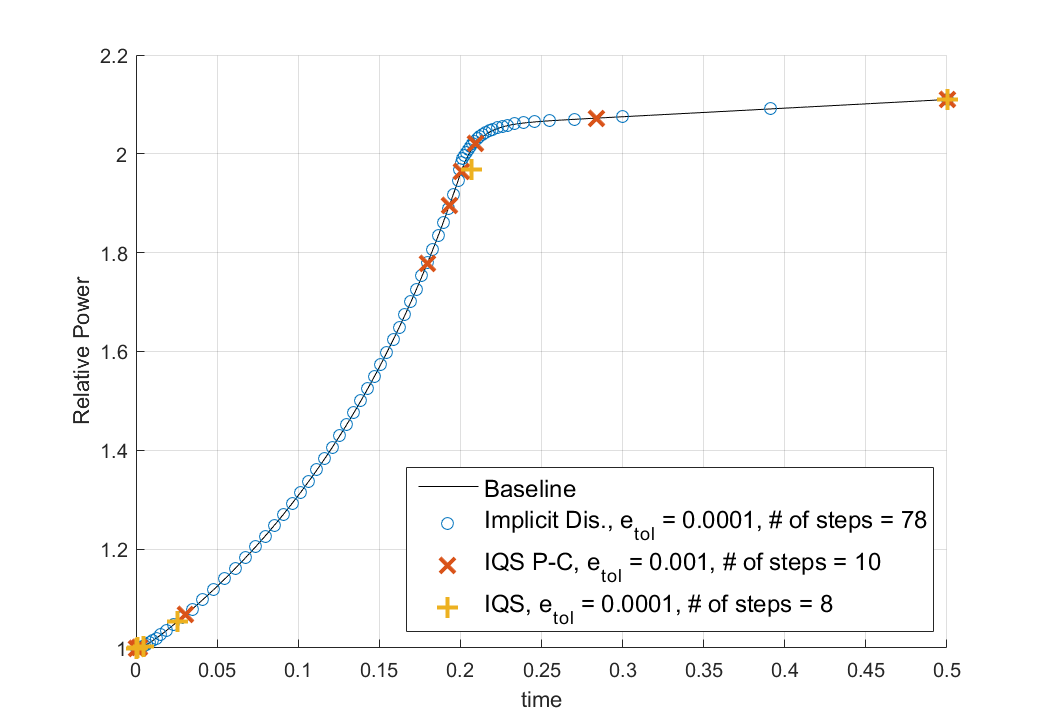
\includegraphics[width=0.8\linewidth]{\FiguresDir/TWIGL_power_plot_dt2.png}
\caption{Power level comparison of TWIGL Benchmark with time adaptation}
\label{fig:TWIGL_power_dt2}
\end{figure}

\newpage

%%%%%%%%%%%%%%%%%%%%%%%%%%%%%%%%%%%%%%%%%%%%%%%%
\subsection{LRA Benchmark}
%%%%%%%%%%%%%%%%%%%%%%%%%%%%%%%%%%%%%%%%%%%%%%%%

The LRA benchmark is a two-dimensional, two-group neutron diffusion problem with adiabatic heat-up and Doppler feedback in thermal reactor \cite{ANL_BPB}.  It is a super prompt-critical transient.  To have better understanding on the cross sections given later, we present the equations here:
\begin{align}
-\frac{1}{v_1} \frac{\partial \phi_1}{\partial t} &= -\grad D_1 \grad\phi_1 + (\Sigma_{a,1} + \Sigma_{s, 1\rightarrow 2})\phi_1 - \nu(1-\beta)S_f  - \sum_{i=1}^2 \lambda_i C_i, \\
-\frac{1}{v_2} \frac{\partial \phi_2}{\partial t} &= -\grad D_2 \grad\phi_1 + \Sigma_{a,2}\phi_2 - \Sigma_{s, 1\rightarrow 2}\phi_1, \\
S_f &= \sum_{g=1}^2 \Sigma_{f,g} \phi_g, \\
\frac{\partial C_i}{\partial t} &= \nu\beta_i f - \lambda_i C_i, \quad i=1,2, \\
\frac{\partial T}{\partial t} &= \alpha f, \label{eq:lra-temp} \\
\Sigma_{a,1} &= \Sigma_{a,1}(\vec{r}, t=0) \left[1+\gamma\left(\sqrt{T} - \sqrt{T_0}\right)\right], \\
P &= \kappa S_f,
\end{align}
where $\phi_1$, $\phi_2$ are the fast and thermal fluxes; $v_1, v_2$ are the averaged neutron velocities; $\Sigma_{a,1}, \Sigma_{a,2}$ are the absorption cross sections; $\Sigma_{s,1\rightarrow 2}$ is the fast-to-thermal scattering cross section; $\Sigma_{f,1}, \Sigma_{f,2}$ are the fission cross sections; $\nu$ is the averaged number of neutrons emitted per fission; $\beta_1, \beta_2$ are the delayed neutron precursor fractions and $\beta=\beta_1 + \beta_2$; $C_1, C_2$ are the delayed neutron precursor concentrations; $\lambda_1, \lambda_2$ are the decay constants of the delayed neutron precursors; $S_6f$ is the fission reaction rate; $P$ is the power density; $T$ is the temperature; $\kappa$ is the averaged power released per fission; $\alpha$ is the combination of $\kappa$ and the specific heat capacity; $\gamma$ is the Doppler feedback coefficient; $T_0=T(\vec{r}, t=0)$.
The two-group diffusion equation are solved with zero flux boundary conditions on external surfaces, reflecting conditions at symmetry boundaries and steady state initial conditions which are obtained by solving
\begin{align}
-\grad D_1 \grad\phi_1 + (\Sigma_{a,1} + \Sigma_{s, 1\rightarrow 2})\phi_1 &= \frac{1}{k}\sum_{g=1}^2 \nu\Sigma_{f,g}\phi_g, \\
-\grad D_2 \grad\phi_1 + \Sigma_{a,2}\phi_2 =& \Sigma_{s, 1\rightarrow 2}\phi_1. \\
\end{align}
The eigenvalue $k$ is used to modify the fission cross section for the transient simulations with $\frac{1}{k}\Sigma_{f,g}, g=1,2$.  The initial flux distribution shall be normalized such that the averaged power density
\begin{align}
\bar{P} \equiv \frac{\int_{V_{core}} P(\vec{r}, t=0) d\vec{r}}{\int_{V_{core}} d\vec{r}},
\end{align}
where $V_{core}$ is the core region with fuels, is equal to $10^{-6} W\cdot cm^{-3}$.
The initial precursor concentrations are in equilibrium with the initial critical flux distribution.\\

The geometry is illustrated in~\fig{fig:lra-geometry}.\\
\begin{figure}[!htbp]
\centering
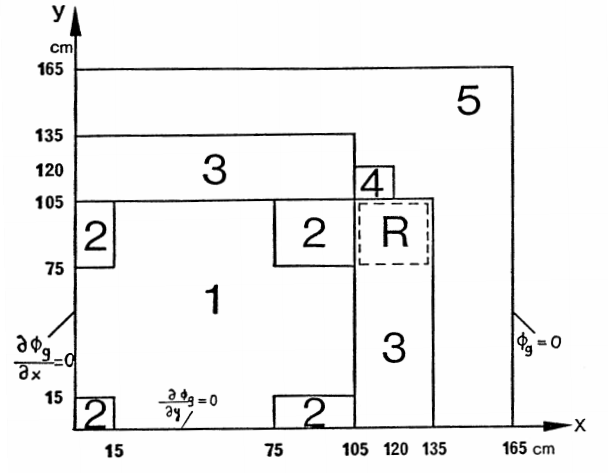
\includegraphics[width=0.8\linewidth]{\FiguresDir/lra.png}
\caption{LRA benchmark geometry with region assignment.}
\label{fig:lra-geometry}
\end{figure}

Initial two-group constants are presented in~\tbl{tab:lra-xs}.
$\nu$ is equal to 2.43.
Axial bulking $B^2 = 10^{-4}$ is applied for both energy groups.
Delayed neutron data are presented in~\tbl{tab:lra-dnp}.
All fuel materials have the same delayed neutron data.
Some scalar data are listed in~\tbl{tab:lra-scalar}.\\
\begin{table}[!htbp]
    \centering
    \caption{LRA benchmark initial two-group constants.\label{tab:lra-xs}}
    \resizebox{\textwidth}{!}{
      \begin{tabular}{|c|c|c|c|l|l|l|l|l|}
      \hline
             &                 & Group   & $D_g$      & $\Sigma_{a,g}$ & $\nu\Sigma_{f,g}$ & $\Sigma_{s,1\rightarrow 2}$ & $\chi_g$ & $v_g$              \\
      Region & Material        &       g & (cm)       &  ($cm^{-1}$)   &  ($cm^{-1}$)      &  ($cm^{-1}$)                &          & ($cm\cdot s^{-1}$) \\
      \hline
      1      & Fuel 1 with rod & 1       & 1.255      & 0.008252       & 0.004602          &                             & 1        & $3.0\times10^7$    \\
             &                 & 2       & 0.211      & 0.1003         & 0.1091            & 0.02533                     & 0        & $3.0\times10^5$    \\
      \hline
      2      & Fuel 1 without rod & 1    & 1.268      & 0.007181       & 0.004609          &                             & 1        & $3.0\times10^7$    \\
             &                    & 2    & 0.1902     & 0.07047        & 0.08675           & 0.02767                     & 0        & $3.0\times10^5$    \\
      \hline
      3      & Fuel 2 with rod & 1       & 1.259      & 0.008002       & 0.004663          &                             & 1        & $3.0\times10^7$    \\
             &                 & 2       & 0.2091     & 0.08344        & 0.1021            & 0.02617                     & 0        & $3.0\times10^5$    \\
      \hline
      4      & Fuel 2 without rod & 1    & 1.259      & 0.008002       & 0.004663          &                             & 1        & $3.0\times10^7$    \\
             &                    & 2    & 0.2091     & 0.073324       & 0.1021            & 0.02617                     & 0        & $3.0\times10^5$    \\
      \hline
      5      & Reflector        & 1      & 1.257      & 0.0006034      & -                 &                             & -        & $3.0\times10^7$    \\
             &                  & 2      & 0.1592     & 0.01911        & -                 & 0.04754                     & -        & $3.0\times10^5$    \\
      \hline
      \end{tabular}}
\end{table}

\begin{table}[!htbp]
    \centering
    \caption{LRA benchmark delayed neutron data.\label{tab:lra-dnp}}
      \begin{tabular}{|c|l|l|l|l|}
      \hline
      Group i & $\beta_i$ & $\lambda_i$ ($s^{-1}$) & $\chi_{d,i,1}$ & $\chi_{d,i,2}$ \\
      \hline
      1       & 0.0054    & 0.0654  & 1 & 0 \\
      2       & 0.001087  & 1.35    & 1 & 0 \\
      \hline
      \end{tabular}
\end{table}

\begin{table}[!htbp]
    \centering
    \caption{LRA benchmark scalar values.\label{tab:lra-scalar}}
      \begin{tabular}{|l|c|l|}
      \hline
      Meaning & Notation & value \\
      \hline
      Axial buckling for both energy groups & $B_g^2$  & $10^{-4}$ ($cm^{-2}$)\\
      Mean number of neutrons per fission   & $\nu$    & 2.43 \\
      Conversion factor                     & $\alpha$ & $3.83\times 10^{-11}$ ($K\cdot cm^{3}$) \\
      Feedback constant                     & $\gamma$ & $3.034\times 10^{-3}$ ($K^{1/2}$) \\
      Energy released per fission           & $\kappa$ & $3.204\times 10^{-11} $ ($J/fission$) \\
      Initial and reference temperature     & $T_0$    & 300 (K) \\
      Active core volume                    & $V_{core}$ & 17550 ($cm^2$)\\
      \hline
      \end{tabular}
\end{table}


The transient is initiated by changing the thermal absorption cross section as the following:
\begin{align}
\Sigma_{a,2}(t) = \Sigma_{a,2}(t=0) \left\{\begin{array}{lr} 1-0.0606184t, & t\leq 2 \\
                                                             0.8787631, & t>2
                                           \end{array}\right.
\end{align}
where $t$ is time in seconds.\\

Figure \ref{fig:LRA_plots} show the IQS  solution as compared with the Brute Force solution.    These plots show that IQS is consistent with Doppler feedback problems in Rattlesnake.  Figure \ref{fig:lra_conv} plots the error convergence of IQS and the Brute Force methods. Table  \ref{tab:LRAdt2} shows the time adaptation performance of both methods.  These results show that IQS, again, performs much better than the brute force method by taking significantly less diffusion solves while retaining similar accuracy.

\begin{figure}[!htbp]
\begin{center}
\begin{subfigure}[!htbp]{0.49\textwidth}
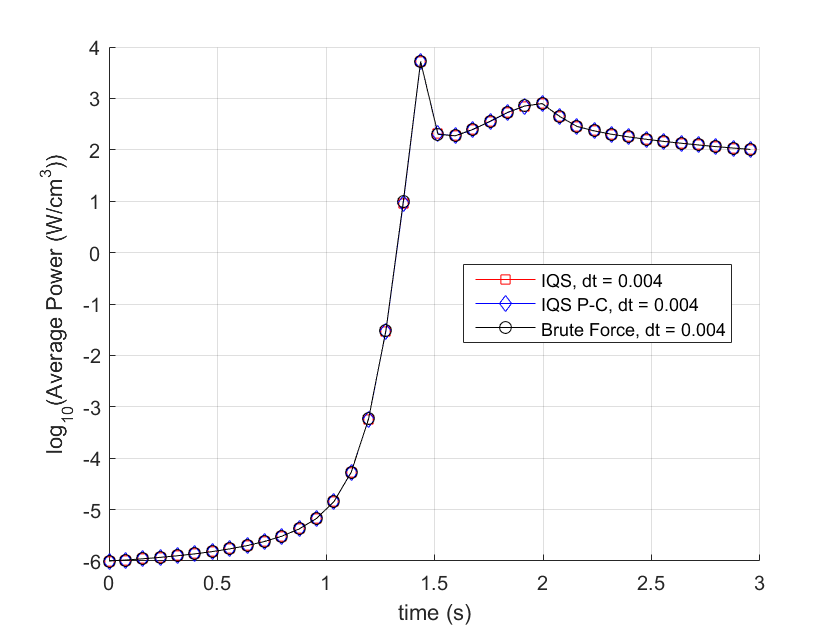
\includegraphics[width=\textwidth]{\FiguresDir/lra_power_profile.png}
\caption{Power Profile}
\end{subfigure}
\begin{subfigure}[!htbp]{0.49\textwidth}
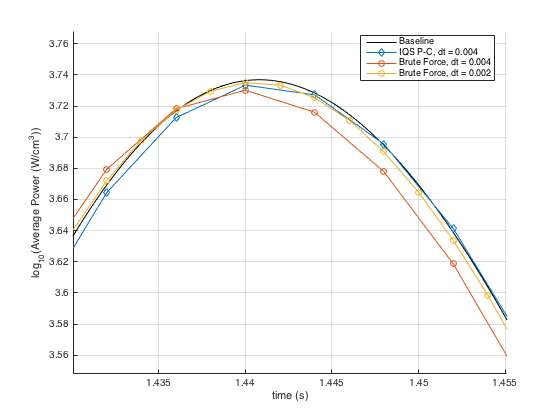
\includegraphics[width=\textwidth]{\FiguresDir/lra_power_profile2.png}
\caption{Power Profile at Peak}
\end{subfigure}
\begin{subfigure}[!htbp]{0.49\textwidth}
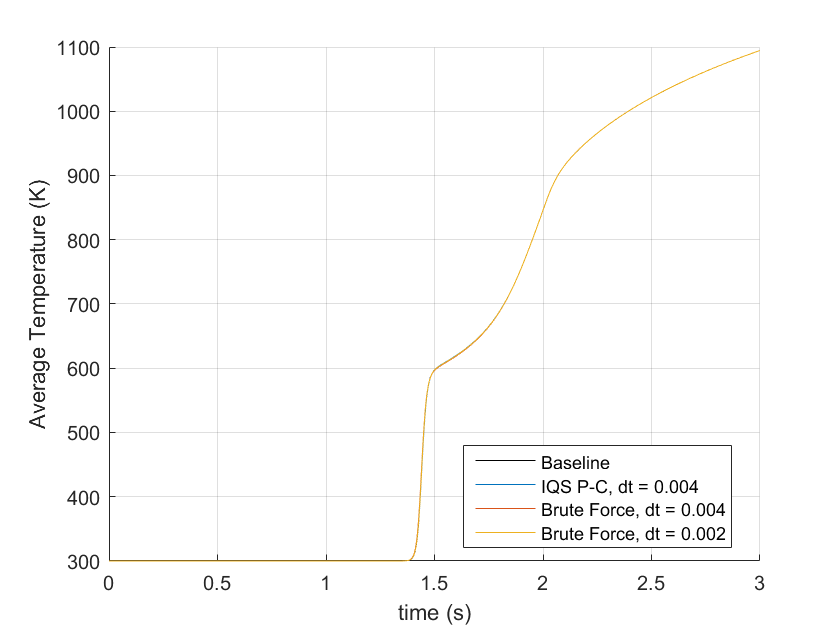
\includegraphics[width=\textwidth]{\FiguresDir/lra_temp_profile.png}
\caption{Temperature Profile}
\end{subfigure}
\caption{LRA Benchmark power and temperature comparison}
\label{fig:LRA_plots}
\end{center}
\end{figure}

\begin{figure}[!htbp]
\centering
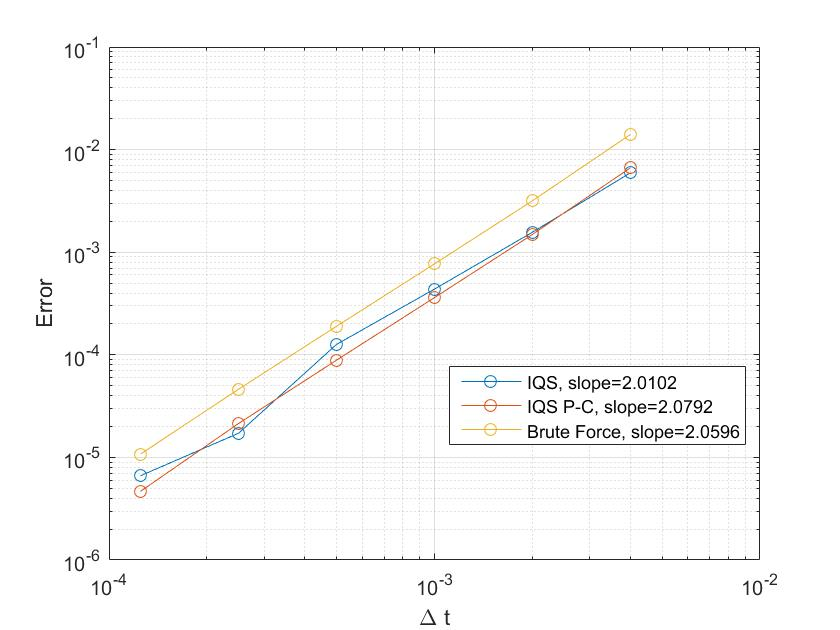
\includegraphics[width=5in]{\FiguresDir/lra_convergence.jpg}
\caption{Error convergence comparison of LRA Benchmark}
\label{fig:lra_conv}
\end{figure}

\begin{table}[!htbp]
\caption{LRA step doubling results}
\label{tab:LRAdt2}
\begin{center}
\begin{tabular}{|l|l|l|l|l|l|l|l|}
\hline
  &  & \multicolumn{3}{|c|}{Brute Force} & \multicolumn{3}{|c|}{IQS P-C} \\
\hline
Test & $e_{max}$ & Error & Steps & Solves & Error & Steps & Solves \\
\hline
1 &	 0.01 &	 0.0437566 &	 145 &	 735 &	 0.143855 &	 105 &	 616 \\ 
2 &	 0.005 &	 0.0309732 &	 266 &	 948 &	 0.104782 &	 157 &	 814 \\ 
3 &	 0.001 &	 0.158242 &	 585 &	 2046 &	 0.155676 &	 218 &	 1062 \\ 
4 &	 0.0005 &	 0.270949 &	 833 &	 2908 &	 0.211994 &	 480 &	 2038 \\ 
5 &	 0.0001 &	 0.280468 &	 1793 &	 6155 &	 0.0437761 &	 434 &	 1458 \\ 
6 &	 5e-05 &	 0.212274 &	 2485 &	 8511 &	 0.0385312 &	 542 &	 1719 \\ 
\hline
\end{tabular}
\end{center}
\end{table}

%%%%%%%%%%%%%%%%%%%%%%%%%%%%%%%%%%%%%%%%%%%%%%%%
%%%%%%%%%%%%%%%%%%%%%%%%%%%%%%%%%%%%%%%%%%%%%%%%
\section{Conclusions}

\tcr{needed}

%%%%%%%%%%%%%%%%%%%%%%%%%%%%%%%%%%%%%%%%%%%%%%%%
%%%%%%%%%%%%%%%%%%%%%%%%%%%%%%%%%%%%%%%%%%%%%%%%

\clearpage
\pagebreak
\newpage
%%%%%%%%%%%%%%%%%%%%%%%%%%%%%%%%%%%%%%%%%%%%%%%%%%%%%%%%%%%%%%%%%%%%%%%%%%%%%
%%%%%%%%%%%%%%%%%%%%%%%%%%%%%%%%%%%%%%%%%%%%%%%%%%%%%%%%%%%%%%%%%%%%%%%%%%%%%
\appendix
%%%%%%%%%%%%%%%%%%%%%%%%%%%%%%%%%%%%%%%%%%%%%%%%%%%%%%%%%%%%%%%%%%%%%%%%%%%%%
%%%%%%%%%%%%%%%%%%%%%%%%%%%%%%%%%%%%%%%%%%%%%%%%%%%%%%%%%%%%%%%%%%%%%%%%%%%%%

%%%%%%%%%%%%%%%%%%%%%%%%%%%%%%%%%%%%%%%%%%%%%%%%%%%%%%%%%%%%%%%%%%%%%%%%%%%%%%
%\section{Appendix: aaaa}
%%%%%%%%%%%%%%%%%%%%%%%%%%%%%%%%%%%%%%%%%%%%%%%%%%%%%%%%%%%%%%%%%%%%%%%%%%%%%%
%
%%%%%%%%%%%%%%%%%%%%%%%%%%%%%%%%%%%%%%%%%%%%%%%%%%%%%%%%%%%%%%%%%%%%%%%%%%%%%%
%\tcr{putting stuff here for now}
%%%%%%%%%%%%%%%%%%%%%%%%%%%%%%%%%%%%%%%%%%%%%%%%%%%%%%%%%%%%%%%%%%%%%%%%%%%%%%
%
%It can be shown that the most appropriate weighting function $(w^g)$ is the initial adjoint flux $(\phi^{*g})$.  For brevity, the following definition will be applied: $\int_D\phi^{*g}(\vec{r})f(\vec{r})d^3r=\left(\phi^{*g},f\right)$
%\begin{align}
%& \quad \frac{dp}{dt}\sum_{g=1}^G\left(\phi^{*g},\frac{1}{v^g}\varphi^g\right)+ p\frac{d}{dt}\sum_{g=1}^G\left(\phi^{*g},\frac{1}{v^g}\varphi^g\right)= \nonumber \\
%& p\sum_{g=1}^G\left(\phi^{*g},\frac{\chi_p^g}{\keff}(1-\beta) \sum_{g'=1}^G  \nu^{g'} \Sigma_f^{g'} \varphi^{g'} + \sum_{g'\neq g}^G\Sigma_s^{g'\to g} \varphi^{g'} - \left( -\div D^g \grad  + \Sigma_r^g \right) \varphi^g\right)  \\
%& + \sum_{i=1}^I\sum_{g=1}^G(\phi^{*g},\chi_{d,i}^g\lambda_i C_i) \nonumber
%\end{align}
%\be
%\frac{d}{dt}\sum_{g=1}^G(\phi^{*g},\chi_{d,i}^gC_i)=\frac{1}{\keff}\sum_{g=1}^G(\phi^{*g},\chi_{d,i}^g\beta_i\sum_{g'=1}^G\nu^{g'} \Sigma_f^{g' }\varphi^{g'})p - \sum_{g=1}^G(\phi^{*g},\chi_{d,i}^g\lambda_iC_i) \quad 1 \le i \le I 
%\ee
%
%In order to impose uniqueness of the factorization, one imposes:
%\be
%\sum_{g=1}^G\left(\phi^{*g},\frac{1}{v^g}\varphi^g\right)=constant
%\ee
%
%Therefore the PRKE formulation reduces to:
%\begin{align}
%\frac{dp}{dt}= &\frac{\sum_{g=1}^G\left(\phi^{*g},\frac{\chi_p^g}{\keff}(1-\beta) \sum_{g'=1}^G  \nu^{g'} \Sigma_f^{g'} \varphi^{g'} + \sum_{g'\neq g}^G\Sigma_s^{g'\to g}  \varphi^{g'} - \left( -\div D^g \grad  + \Sigma_r^g \right) \varphi^g\right)}{\sum_{g=1}^G\left(\phi^{*g},\frac{1}{v^g}\varphi^g\right)}p \nonumber \\ 
%& +\sum_{i=1}^I\frac{\sum_{g=1}^G(\phi^{*g},\chi_{d,i}^g\lambda_i C_i)}{\sum_{g=1}^G(\phi^{*g},\chi_{d,i}^gC_i)}\xi_i
%\end{align}
%\be
%\frac{d\xi_i}{dt}=\frac{1}{\keff}\frac{\sum_{g=1}^G(\phi^{*g},\chi_{d,i}^g\beta_i\sum_{g'=1}^G\nu^{g'} \Sigma_f^{g' }\varphi^{g'})}{\sum_{g=1}^G\left(\phi^{*g},\frac{1}{v^g}\varphi^g\right)}p - \frac{\sum_{g=1}^G(\phi^{*g},\chi_{d,i}^g\lambda_iC_i)}{\sum_{g=1}^G(\phi^{*g},\chi_{d,i}^gC_i)}\xi_i \quad 1 \le i \le I 
%\ee
%Where:
%\be
%\xi_i=\frac{\sum_{g=1}^G(\phi^{*g},\chi_{d,i}^g C_i)}{\sum_{g=1}^G\left(\phi^{*g},\frac{1}{v^g}\varphi^g\right)}
%\ee
%
%It is convenient to define the effective reactivity, delay-neutron fraction, and delayed-neutron precursor decay constant:
%\be
%\frac{\rho-\bar{\beta}}{\Lambda}=\frac{ \sum_{g=1}^G\left(\phi^{*g},\frac{\chi_p^g}{\keff}(1-\beta)\sum_{g'=1}^G \nu^{g'} \Sigma_f^{g'}\varphi^{g'} + \sum_{g'\neq g}^G\Sigma_s^{g'\to g} \varphi^{g'} -\left( -\div D^g \grad  + \Sigma_r^g \right)\varphi^g\right)}{\sum_{g=1}^G\left(\phi^{*g},\frac{1}{v^g}\varphi^g\right)}
%%\label{eq:rmb}
%\ee
%\be
%\frac{\bar{\beta}}{\Lambda}=\sum_{i=1}^I\frac{\bar{\beta}_i}{\Lambda}=\sum_{i=1}^I\frac{1}{\keff}\frac{\sum_{g=1}^G(\phi^{*g}, \chi_{d,i}^g\beta_i\sum_{g'=1}^G\nu^{g'} \Sigma_f^{g' }\varphi^{g'})}{\sum_{g=1}^G\left(\phi^{*g},\frac{1}{v^g}\varphi^g\right)}
%%\label{eq:b}
%\ee
%\be
%\bar{\lambda}_i=\frac{\sum_{g=1}^G(\phi^{*g},\chi_{d,i}^g\lambda_i C_i)}{\sum_{g=1}^G(\phi^{*g},\chi_{d,i}^gC_i)}
%%\label{eq:l}
%\ee
%
%So:
%\be
%\frac{dp}{dt}=\left[\frac{\rho-\bar{\beta}}{\Lambda}\right]p+\sum_{i=1}^I\bar{\lambda}_i\xi_i
%%\label{eq:p}
%\ee
%\be
%\frac{d\xi_i}{dt}=\frac{\bar{\beta}_i}{\Lambda}-\bar{\lambda}_i\xi_i \quad 1 \le i \le I 
%%\label{eq:c}
%\ee
%
%Equations (\ref{eq:p}) and (\ref{eq:c}) are a formulation of the point reactor kinetics equation (PRKE), but the parameters (Equations (\ref{eq:rmb})-(\ref{eq:l})) are dependent on the shape.  If the assumption is made that the shape is time-independent, the shape is computed once at the first time step and used for the PRKE parameter evaluation at all other steps.  However, if the shape is dependent on time, the shape needs to be computed in transient using equation (\ref{eq:shape}) and (\ref{eq:prec}) in order retain accuracy.  Equations (\ref{eq:shape2}) and (\ref{eq:preq2}) shows the usual form of the shape and precursor equations with amplitude put on the right hand side.  Equation (\ref{eq:shape2}) is very similar to the multigroup flux equation (\ref{eq:flux}), except the removal cross-section term is augmented by a $\frac{1}{v^g}\frac{1}{p}\frac{dp}{dt}$ term and the precursor contribution has a $\frac{1}{p}$ multiplier.  Equation (\ref{eq:preq2}) is very similar to the normal precursor equation (\ref{eq:precursor}), except the fission source term is multiplied by $p$.  These differences are crucial for IQS implementation in Rattlesnake.
%
%\begin{align}
%\frac{1}{v^g}\frac{\partial\varphi^g}{\partial t} = &\frac{\chi_p^g}{\keff} (1-\beta)\sum_{g'=1}^G  \nu^{g'} \Sigma_f^{g'} \varphi^{g'} + \sum_{g'\neq g}^G\Sigma_s^{g'\to g} \varphi^{g'} \nonumber \\ 
%& -  \left( -\div D^g \grad  + \Sigma_r^g + \frac{1}{v^g}\frac{1}{p}\frac{dp}{dt}\right) \varphi^g + \frac{1}{p}\sum_{i=1}^I\chi_{d,i}^g\lambda_iC_i  , \quad 1 \le g \le G 
%%\label{eq:shape2}
%\end{align}
%\be
%\frac{dC_i}{dt} = \frac{\beta_i}{\keff}p \sum_{g=1}^G\nu^{g} \Sigma_f^g \varphi^{g} - \lambda_i C_i \ , \quad 1 \le i \le I 
%%\label{eq:preq2}
%\ee

%\begin{align}
%& \quad \sum_{g=1}^G\left(\phi^{*g},\frac{1}{v^g}\frac{\partial\varphi^g}{\partial t}\right)= \nonumber \\ 
%&\sum_{g=1}^G\left(\phi^{*g},\frac{\chi_p^g}{\keff} \sum_{g'=1}^G (1-\beta) \nu^{g'} \Sigma_f^{g'} \varphi^{g'} + \sum_{g'\neq g}^G\Sigma_s^{g'\to g} \varphi^{g'} -  \left( -\div D^g \grad  + \Sigma_r^g + \frac{1}{v^g}\frac{1}{p}\frac{dp}{dt}\right) \varphi^g\right) \\
%&+\frac{1}{p}\sum_{i=1}^I\sum_{g=1}^G(\phi^{*g},\chi_{d,i}^g\lambda_iC_i) \nonumber
%\end{align}

%%%%%%%%%%%%%%%%%%%%%%%%%%%%%%%%%%%%%%%%%%%%%%%%%%%%%%%%%%%%%%%%%%%%%%%%%%%%%%%%
\bibliographystyle{abbrvnat}
\bibliography{references_IQS}
\end{document}